\documentclass[12pt,french]{report}
\usepackage{graphicx}\usepackage{longtable}
\usepackage{fmtcount}
\usepackage{textcomp}
\usepackage{txfonts}
\usepackage{makeidx}
\usepackage{multirow}\usepackage{multicol}
\usepackage{plain}
\usepackage{algorithm,algorithmic}
\usepackage{pdfpages}
\usepackage[toc,page]{appendix}
\usepackage[french]{babel}\RequirePackage[T1]{fontenc}
\selectlanguage{french}
\usepackage[utf8]{inputenc}

\usepackage[nottoc, notlof, notlot]{tocbibind}
\usepackage{lscape}
\usepackage[left=3cm,right=2cm,top=2cm,bottom=3cm]{geometry}
\usepackage{url}
\usepackage{float}
\usepackage{bibentry}
\usepackage{xcolor,colortbl}
\usepackage{rotating}
\usepackage{caption}
\usepackage{longtable}
\usepackage{verbatim}
%\usepackage{supertabular}

\begin{document}
 \begin{center}
\thispagestyle{empty}
\vspace{-3cm}
\center{\textsc{Minisètre de l'Enseignement Supérieur Et de la Recherche Scientifique}}\vspace{-0.3cm}
\center{\textsc{Université de Tunis}}
\vspace{-0.3cm}
\center{\textsc{Institut Supérieur de Gestion}}
\begin{figure} [H]
\begin{center}

\includegraphics [width=2.5cm]{figures/logoisg.pdf}
\hspace{3.5cm}

\includegraphics [width=4cm]{figures/linedatalogo.png}
\end{center}
\end{figure}
\vspace{-0.5cm}





\vspace{1cm}

\center{\textbf{\large{TABLEAU DE BORD DE SUIVI ET AUTOMATISATION DES PLANNINGS D'UN PROJET}}} % en maj
\vspace{0.9cm}
\center{\textbf{\large{Linedata}}}
\vspace{1cm}


\center{\large{\textsc{\textbf{Elaboré par}}}}\\
\center{\large{Mohamed Ali Touir}} %If solo and delete the code related to minipage
%\vspace{0.5cm}
%\begin{minipage}{12cm}
 %\begin{center}
 %Mohamed Ali Touir
 %\end{center}
%\end{minipage}

\vspace{1.5cm}
\center{\large{\textsc{\textbf{Filière}}}}
\center{Licence Fondamentale en Informatique de Gestion}

\vspace{1.5cm}
\center{\large{\textsc{\textbf{Encadré par}}}}
\vspace{0.5cm}

 \begin{minipage}{6cm}
 \begin{center}
 \textbf{Encadrant pédagogique}   \\ Mlle. Zeineb Chelly
 \end{center}
\end{minipage}
\begin{minipage}{6cm}
\begin{center}
\textbf{Encadrant professionnel} \\Mr. Adnen Sadfi
\end{center}
 \end{minipage}

 \vspace{2cm}

 \begin{center}
\footnotesize{Année universitaire} \\ \footnotesize{2016-2017}
\end{center}







\end{center}
 %vous utilisez le fichier PageGardeCo.tex si vous avez un Co-encadrant p\'{e}dagogique. Sinon, vous utilisez le fichier PageGarde.tex
 \setcounter{page}{1} \pagenumbering{roman}
\chapter*{Dédicaces}
Je dédis ce travail:\\

À ma famille, mes amis et mes collègues qui m'ont encouragé et soutenu tout au long de la réalisation du projet.\\

À tous ceux qui m'ont aidé dans la société ou en ligne et dans les forums et qui m'ont fourni l'aide et les outils ou bibliothèques tierces nécessaires à la réalisation du projet.

\begin{flushright}
Mohamed Ali Touir
\end{flushright}
\newpage
\chapter*{Remerciements}
Au terme de ce travail, je tiens à exprimer ma gratitude et mes remerciements pour toutes les personnes qui ont contribué à sa réalisation.\\

Tout d’abord, j'adresse mes remerciements à \textbf{Mademoiselle Zaineb Chelly} pour m'avoir accompagné durant toutes les étapes de la réalisation du projet. Ses conseils, son soutien et son sens du sérieux m'ont permis de faire face aux difficultés rencontrées et d’aboutir à un projet réussi.\\

Je remercie également \textbf{Monsieur Adnen Sadfi}, \textbf{Monsieur Ghazi Souelmi} et \textbf{Mademoiselle Ons Bouzouida} pour m'avoir donné l’opportunité de travailler sur ce projet. Cette expérience m'a permis d’acquérir des connaissances techniques et m'a fait découvrir la vie professionnelle en me traitant comme étant un employé et non pas un externe.\\

Enfin, je tiens à remercier toute personne qui à cru en moi, qui m'a encouragé et qui m'a inspiré durant les moments fastidieux de ce projet.
\newpage
\listoffigures
\newpage
 \listoftables
\newpage
\tableofcontents
\newpage

 \pagestyle{headings}
 \setcounter{page}{1}
\pagenumbering{arabic}
\addcontentsline{toc}{chapter}{Introduction générale}
\chapter*{Introduction générale}
Le domaine de gestion de projet grandi de plus en plus et ceci à cause d'un besoin critique qui est présent depuis l'apparition des civilisations. Quel que soit le projet, vous rencontrerez toujours les mêmes contraintes :\\
\begin{itemize}
    \item[$\bullet$] Qualité: votre produit doit répondre aux attentes
    \item[$\bullet$] Délai: votre produit doit être livré dans les délais
    \item[$\bullet$] Coûts: la réalisation du projet ne doit pas dépasser les limites budgétaires.\\
\end{itemize}

Ces derniers sont liés et chaque action sur l'un entraîne des répercussions sur les autres. Si on réduit les délais, il faut soit augmenter les coûts en mettant plus de mains-d'œuvre sur le projet, soit de réduire la qualité du produit pour finir dans les temps. Et ceci sans parler des imprévus. Sur ce, il faut une excellente planification du projet et une bonne gestion de risque pour le bon déroulement du projet.\\

Un chef de projet est un membre de l'équipe qui gère tous ces contraintes. Pour cela, il doit non seulement avoir des connaissances techniques de base, mais en plus il doit connaître les compétences des membres de son équipe. Et ceci pour pouvoir calculer le temps nécessaire pour finir un scénario ou une tâche dans un projet et pouvoir distribuer les tâches sur les membres.\\

Dans le cadre de mon projet de fin d'études et dans cet aspect, Linedata m'a proposé le sujet intitulé "Tableau de bord de suivi et automatisation des plannings d'un projet". Cette dernière a voulu faciliter la tâche d'un chef d'équipe en automatisant quelques traitements qu'il fait et en mettant à sa disposition des tableaux de bords pour avoir une vue globale sur le rendement de son équipe.\\

Notre projet de fin d'études comporte les chapitres suivants:\\
\begin{itemize}
    \item[$\circ$] Le premier chapitre "Cadre général du projet", présente l'organisme d'accueil, la méthodologie de travail utilisé et le contexte du projet.
    \item[$\circ$] Le deuxième chapitre "Analyse des besoins", présente les acteurs et besoins du projet en plus du backlog produit et la planification de release.
    \item[$\circ$] Le troisième chapitre "Conception et réalisation de l'application", présente l'environnement de travail et les choix architecturaux.
    \item[$\circ$] Le quatrième chapitre "Organisation des sprints", présente la réalisation du projet.\\
\end{itemize}
Et nous finirons le rapport par une conclusion générale et la bibliographie.
\chapter{Cadre général du projet}
\section{Introduction}
Dans ce chapitre, nous allons présenter le cadre du projet. En premier lieu, nous proposerons une présentation de l'entreprise d'accueil Linedata. Ensuite nous présenterons une critique de la solution existante ainsi que les solutions proposées. Et nous clôturons ce chapitre par une exposition de la méthodologie suivie tout au long de la réalisation du projet.
\section{Présentation de l'organisme d'accueil}
Linedata est un éditeur de solutions globales qui travaille dans le secteur de management, de l'assurance et du crédit. Chaque jour, plus de 63000 professionnels financiers opérant dans 50 pays font confiance à ses technologies afin de gérer leurs activités. Le logo de l'organisme d'accueil est présenté par la Figure \ref{code1}
\begin{figure}[h]
  \centering
  
\includegraphics[scale=0.3]{figures/linedatalogo.png}
  \caption{Logo Linedata}
  \label{code1}
\end{figure}

\subsection{Historique}
Linedata est né en janvier 1998 du rapprochement de trois sociétés: \textbf{Générale de service informatique (GSI) Division des Banques}, \textbf{Line Data} et \textbf{BDB Participation}.\\

GSI Division des banques a été rachetée majoritairement par ses salariés au mois de décembre 1997. L'accquisition ultérieure de Line Data et de BDB Participation a permis la constition d'une nouvelle société: \textbf{Linedata Services}.

Cette dernière n'est pas donc une création de toutes pièces mais elle avait dès ses débuts du savoir-faire humain et technologique ce qui lui a permis en 17 mai 2000 d'être introduit en bourse sur le Nouveau Marché de la Bourse de Paris. Linedata est ainsi depuis 10 ans une société cotée sur Euronext Paris.\\

Linedata s'est rapidement développé pour accompagner ses clients en élargissant son offre produit tout en ciblant de nouveaux marchés. Afin d'accompagner sa croissance, Linedata a mis en place une stratégie d'acquisition et d'intégration réussie depuis plus de 15 ans:\\
\begin{itemize}
    \item[$\bullet$] Février 2000: Les sociétés Bimaco Finance, Pen Lan et EKIP/Ingénétudes qui sont basées à Paris ont permis à Linedata d'appuyer sa leadership dans le domaine des crédits et financement.\\
    \item[$\bullet$] Février 2003: Acquisition des solutions Icon et Préview qui permettent la gestion de protefeuilles. Ils ont permis au groupe de rejoindre la tête du classement au Royaume-Uni et de consolider sa position de numéro 1 en Europe.\\
    \item[$\bullet$] Décembre 2003: Acquisition de Economic and Social Data Service Solutions (ESDS) qui est un des spécialistes français dans le domaine des progiciels d'assurance individuelle. Ceci a permis à Linedata Services d'être en 2004 un acteur majeur dans le domaine d'Epargne Retraite et la Prévoyance tout en se positionnant significativement sur le segment en très forte croissance des assurances de personnes.\\
    \item[$\bullet$] Mars 2013: Acquisition de l'activité CapitalStream auprès de  Hindustan Computers Limited Technologies (HCL), basée à Seattle et à Irvine, qui a permis à Linedata d'offrir une solution globale front to back sur les marchés des crédits et financements en Amérique du Nord et en Europe.\\
    \item[$\bullet$] Avril 2016: Acquisition de Derivation qui est l'acteur du tout premier plan spécialisé dans la gestion des risques, les données analytiques et la gestion de portefeuille pour les gérants institutionnels et alternatifs à l'échelle mondiale. Cette dernière a permis à Linedata de proposer désormais une plate-forme globale et complète sur toute la chaîne d'investissement de ses clients, et ce pour tout type d'actif et tout type de structure.\\
\end{itemize}
Linedata a su acquérir et intégrer de nombreuses sociétés en quelques années. Cette politique pro-active lui permet d'accompagner ses clients à travers des solutions Front to Back intégrées et modulaires pour les professionnels de la gestion d'actifs, de l'assurance et du crédit \cite{LinedataHistoire}.
\subsection{Domaines d'expertise}
Linedata est un prestataire de solutions mondial et indépendant dédié à la communauté internationale des professionnels de l'Asset Management et du Crédit. Ayant plus de 900 collaborateurs répartis dans le monde, Linedata comprend les enjeux de ses clients et leur propose des solutions et des services innovants et adaptés à l'évolution de leur cœur de métier. Linedata met à disposition le meilleur de la technologie logicielle et du service pour répondre aux besoins des:\\
\begin{itemize}
    \item[$\bullet$] Sociétés de gestion et intermédiaires financiers: Sociétés de gestion de protefeuilles institutionnels et collectifs, administrateurs de fonds, agents de transfert, teneurs de compte d'épargne entreprise, filiales de banques ou indépendants. Linedata propose toute une gamme de produits pour gérer l'ensemble des processus d'investissement.\\
    \item[$\bullet$] Compagnies d'assurance et mutuelles, caisses de retraite et instituts de prévoyance: Linedata propose un progiciel unique sur le marché européen permettant de gérer tous les types de contrats d'assurance de personnes depuis l'épargne individuelle jusqu'à la prévoyance en passant par la retraite collective.\\
    \item[$\bullet$] Entreprises commerciales et industrielles: Linedata intervient après des moyennes et grandes sociétés pour la gestion de leur actionnarriat salarié.\\
    \item[$\bullet$] Etablissements de crédits spécialisés: Linedata met à la disposition de ces spécialistes financiers une solution progicielle unique, globale et reconnue qui couvre l'ensemble des activités de crédit et de financement des particuliers ou des entreprises \cite{LinedataSolutions}.\\
\end{itemize}
\subsection{Présentation de Linedata Tunisie}
Linedata Services (LDS) Tunisie s'est installée à Tunis en 2000 et elle compte actuellement 300 employés. Elle a choisi de se spécialiser dans les domaines Epargne et Assurance, Crédit et Financement.\\

On remarque que Linedata Tunisie se décompose en sept grands départements. Executive Assistance est le bureau des directeurs et dirigeants de la société. Ensuite vient celui des Ressources humaines qui est chargé des recrutements. En troisième est le bureau Maintenance qui est chargé du maintien du matériel au sein de la société. En retrouve après le bureau TM qui est décomposé en Information sécurity qui est chargé des contrôles de sécurité dans la société et le bureau Corporate IT qui est chargé des réseaux sociaux (publications, annonces). Les deux derniers bureaux sont spécialisés dans les produits et services que propose Linedata que ce soit du développement, de l'assurance qualité ou même de la maintenance et stabilisation. La Figure \ref{code2} représente l'organigramme de LDS.


\begin{figure}[H]
  \centering
  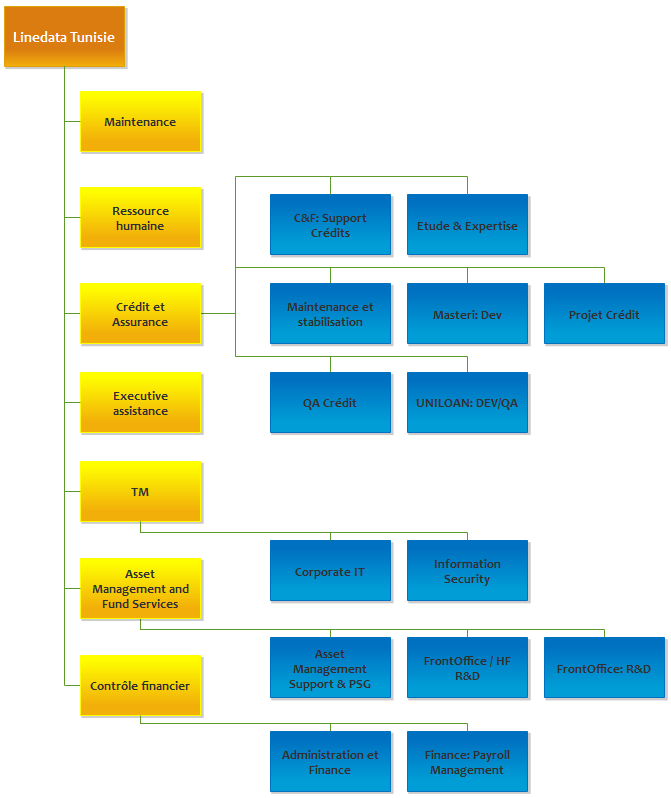
\includegraphics[scale = 1.0]{figures/Organigramme_Linedata_2.png}
  \caption{Organigramme de Linedata Tunisie}
  \label{code2}
\end{figure}


\newpage
\section{Contexte du projet}
Dans cette section, nous allons détailler les objectifs du projet ainsi que les différentes tâches à réaliser.
\subsection{Etude de l'existant}
Linedata est une société qui offre des solutions globales de qualité. De ce fait, cette dernière donne une importance majeure aux avis de ses clients. Chaque jour, elle reçoit de multiples demandes d'ajout de fonctionnalités ou des réclamations de bogue que ce soit du client ou de leurs assurances qualité. Ces réclamations sont donc triées puis distribuées aux équipes chargées de la maintenance du produit concerné. Le chef d'équipe doit alors distribuer les tâches aux membres de son équipe. Pour pouvoir les distribuer, ce dernier doit se baser sur plusieurs indicateurs de performance. Il doit en premier lieu utiliser des requêtes SQL\footnote{Structured Query Language, en français langage de requête structurée.  C'est un langage informatique normalisé servant à exploiter des bases de données relationnelles \cite{SQL}} pour extraire les données nécessaires sur chaque membre de l'équipe d'une base de données déjà existante. La figure \ref{code4} représente un exemple d'une requête SQL utilisée.
\begin{figure}[H]
  \centering
  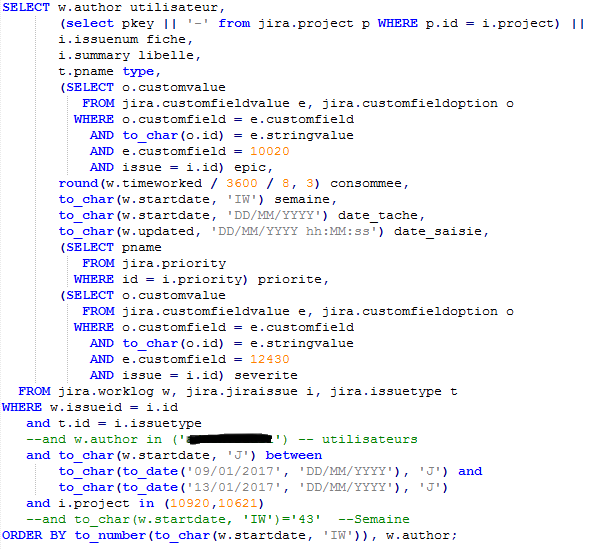
\includegraphics[scale=0.65,width=10cm]{figures/used_sql_request.png}
  \caption{Requête SQL utilisée}
  \label{code4}
\end{figure}
Puis les données sont saisies et enregistrées manuellement sous format Excel. La Figure \ref{code5} représente un exemple de feuille Excel. 
\begin{figure}[H]
  \centering
  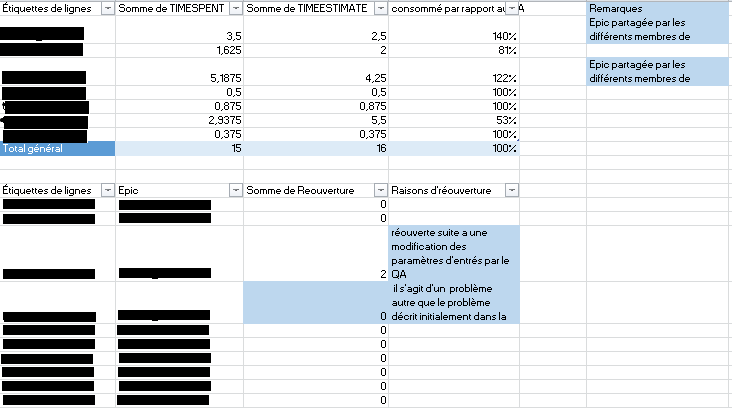
\includegraphics[scale=0.7]{figures/used_excel_file.png}
  \caption{Feuille Excel utilisée}
  \label{code5}
\end{figure}
Ensuite, le chef d'équipe calcule quelques indicateurs de performance à partir de la feuille Excel tel que le nombre de tâches traitées qui ont une certaine complexité sur le nombre de jours passés, le nombre de tâches traitées sur le nombre de jours passés regroupé par mois et le nombre de retours\footnote{Un retour sur une tâche est la non-validation de la tâche traitée et la demande de correction de cette dernière} sur le total des tâches traitées. La figure \ref{code9} représente un exemple de rapport après le calcul de l'indicateur de performance ratio des tâches par mois.
\begin{figure}[H]
  \centering
  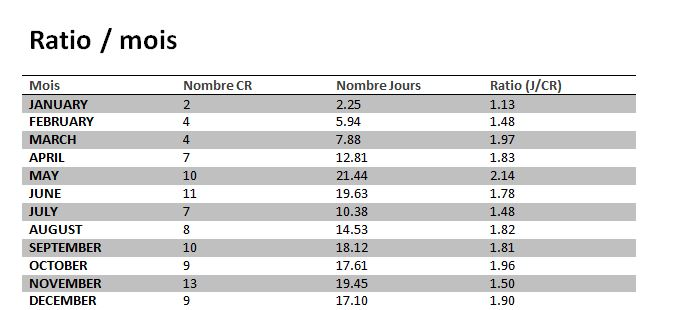
\includegraphics[scale=1.06]{figures/ratio_mois_example.jpg}
  \caption{Exemple de rapport d'indicateurs: Ratio tâches par mois}
  \label{code9}
\end{figure}
Enfin, le chef d'équipe distribue les tâches aux membres en estimant le temps nécessaire pour les finir et en s’appuyant sur les indicateurs de performance.
\subsection{Critique de l'existant}
Le responsable, ne disposant d'aucun outil d'aide pour la collecte et le calcul des indicateurs, mettait trop de temps dans la sélection des membres qui vont s'occuper d'une réclamation. En plus de cela, le risque d'erreur est toujours présent puisque le calcul se faisait de façon manuelle. Sans parler du fait que le suivi du rendement était une tâche difficile puisqu'il n'existe aucun outil de collecte d'informations sur les employés et de traitement de ces derniers dans la société.
\subsection{Présentation du projet}
Afin de faciliter la tâche du chef de projet, nous proposons une solution qui va être décomposée en deux parties: la première qui consiste à créer des tableaux de bords pour le suivi des membres de l'équipe (suivi de performances des membres avec les différents indicateurs de performance évoqués). Ces tableaux de bords vont être basés sur plusieurs indicateurs de performance tels que le nombre de jours passés dans le traitement de fiches regroupé par complexité ou le nombre de fiches traité dans une période déterminée. La seconde partie va tourner autour de l'optimisation des plannings. Et ceci en automatisant le calcul des indicateurs de performance des membres de l'équipe et en optimisant le choix des membres qui vont traiter les tâches.
Cette solution va considérablement réduire le temps que prend l'étape de sélection des membres. Elle va aussi éliminer le risque d’erreurs de calcul et de collecte de données erronées.
\section{Langage de modélisation UML}
La notation UML\footnote{Unified Modeling Language en anglais qui signifie langage de modélisation unifié} est un \textbf{langage visuel} constitué d'un ensemble de schémas, appelé des diagrammes, qui donnent chacun une vision différente du projet à traiter. UML nous permet donc de représenter le logiciel à développer sous forme de diagrammes qui définissent son fonctionnement.\cite{UMLIntroduction}\\

UML est constitué de 13 diagrammes qui représentent chacun un concept du système. Ces derniers peuvent être représentés par le schéma de 4 vues qui est axées sur les besoins des utilisateurs et qu'on appelle 4+1 vues.\\

Les besoins des utilisateurs représente le cœur de l'analyse. On y décrit le contexte, les acteurs du projet, les fonctionnalités et les interactions entre ces acteurs et ces fonctionnalités.
Les besoins peuvent être représentés à l'aide de deux diagrammes: le diagramme de packages et le diagramme de cas d'utilisation.\\

La vue logique a pour but d'identifier les éléments du domaine et les relations et interactions entre ces éléments. Cette vue organise les éléments du domaine en catégories. Deux diagrammes peuvent être utilisés: le diagramme de classes et le diagramme d'objets.\\

La vue des processus démontre la décomposition du système en processus et actions, les interactions entre les processus et la synchronisation et la communication des activités parallèles. La vue des processus peut être représentée par plusieurs diagrammes: le diagramme de séquence, le diagramme d'activité, le diagramme de collaboration, le diagramme d'état-transition, le diagramme global d'interaction et le diagramme de temps.\\

La vue des composants (vue de réalisation) permet de mettre en évidence les composant du futur système(fichiers sources, bibliothèques, base de données ou autre). Cette vue comprend deux diagrammes: le diagramme de structure composite et le diagramme de composants.\\

La vue de déploiement décrit les ressources matérielles et la répartition des parties du logiciel sur ces éléments. Cette vue contient qu'un diagramme: le diagramme de déploiement\cite{UMLDiagrams}.\\

\section{Méthodologie de travail}
Après des recherches sur les méthodes de gestion de projets nous avons choisi les méthodes agiles pour piloter le nôtre.
\subsection{Approche agile}
Le mouvement des méthodes agiles a vu le jour en 2001 aux États-Unis \cite{Agile}. Des experts dans le domaine de l'informatique se sont réunis afin de créer ces méthodes suite à un taux d'échec important des projets informatiques dans les années 1990.\\

Les méthodes agiles se reposent sur des cycles de développement itératifs et incrémentaux en fonction des besoins évolutifs du client. Ces méthodes permettent donc de mieux répondre aux attentes du client en un temps limité (grâce à l'implication de ce dernier) tout en faisant monter les collaborateurs en compétences. Ces méthodes constituent donc un gain en productivité.
Il existe plusieurs méthodes agiles telles que eXtreme Programming(XP), Crystal, Kanban ou encore Rapid Application Development (RAD). Nous avons choisi d'utiliser Scrum pour notre projet.
\subsection{Méthode Scrum}
La méthode Scrum est une méthode agile créée en 2002 dont le nom signifie littéralement "la mêlée". Elle consiste à découper le projet en des itérations qu'on nomme sprints. Un sprint a une durée qui varie entre deux à quatre semaines.
Avant chaque sprint, les tâches sont estimées en temps et en complexité et ceci pour planifier les livraisons et estimer les coûts auprès du client. Les fonctionnalités qui font objet d'un sprint (appelé user stories) constituent ce qu'on appelle sprint backlog du produit qui va être livré à la fin du sprint. Il est nécessaire de distinguer entre sprint backlog et product backlog qui est l'ensemble des fonctionnalités du produit final.\\

La méthode Scrum est caractérisée par une mêlée quotidienne, dans laquelle les membres de l'équipe indiquent les tâches qu'ils ont finies, les difficultés rencontrées et ce qu'il leur reste à faire. Cela permet d'évaluer l'avancement du projet et surtout de venir en aide à ceux qui rencontre des difficultés qu'on a déjà rencontrées auparavant.\\

La figure \ref{code3} présente une itération selon la méthode Scrum
\begin{figure}[H]
  \centering
  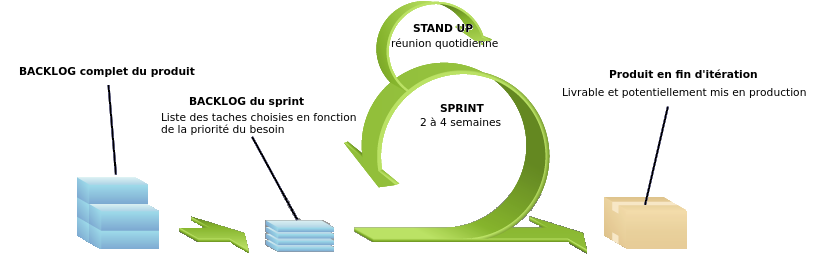
\includegraphics[scale=0.7]{figures/iteration_scrum.png}
  \caption{Itération selon la méthode Scrum}
  \label{code3}
\end{figure}

\subsubsection{Les rôles de la méthode Scrum}
La méthode Scrum définit trois rôles:\\
\begin{itemize}
\item[$\circ$] \textbf{Product Owner}: Il s'agit du représentant du client dans un projet Scrum. Il définit les besoins et les spécifications. Il est aussi chargé de définir les user stories.\\
\item[$\circ$] \textbf{Scrum master}: Il est chargé de veiller à la mise en application de la méthode et le respect de ses objectifs. C'est une personne chargée de lever les obstacles qui ralentissent l'avancement de l'équipe et du projet.\\
\item[$\circ$] \textbf{L'équipe}: Ce sont les personnes chargées de la réalisation des sprints. Il peut s'agir d'un architecte, développeur ou testeur.
\end{itemize}
\section{Conclusion}
Dans ce chapitre nous avons présenté l'organisme d'accueil. Puis, nous avons énoncé le contexte du projet. Après, nous avons défini le langage de modélisation UML et à la fin, nous avons présenté la méthode qu'on va utiliser pour la réalisation du projet. Dans le prochain chapitre, nous allons détailler les besoins de notre projet.
\chapter{Analyse des besoins}
\section{Introduction}
Dans ce chapitre, nous allons présenter l'analyse des besoins. En premier lieu, nous parlerons des besoins et des acteurs qui interviennent dans ce projet. Après, nous proposerons un diagramme de cas d'utilisation globale. Ensuite nous présenterons le backlog produit. Et nous clôturons ce chapitre par une exposition de la planification de release.
\section{Capture des besoins}
Le but de notre application est de collecter des informations de l’outil de gestion
de projet Jira\footnote{Jira est un système de suivi de bugs, un système de gestion des incidents, et un système de gestion de projets développé par Atlassian \cite{Jira}.} pour le calcul des indicateurs et de proposer un planning tenant compte de la performance des
équipes. L’application offrira aussi un tableau de bord de suivi des membres de l'équipe (suivi de
performances des membres).
\subsection{Acteurs}
Un acteur est l'idéalisation d'un rôle joué par une personne externe, un processus ou une chose qui interagit avec un système \cite {Acteur}. Les trois acteurs principaux de notre application sont représenté par la figure \ref{code6}.
\begin{figure}[H]
  \centering
  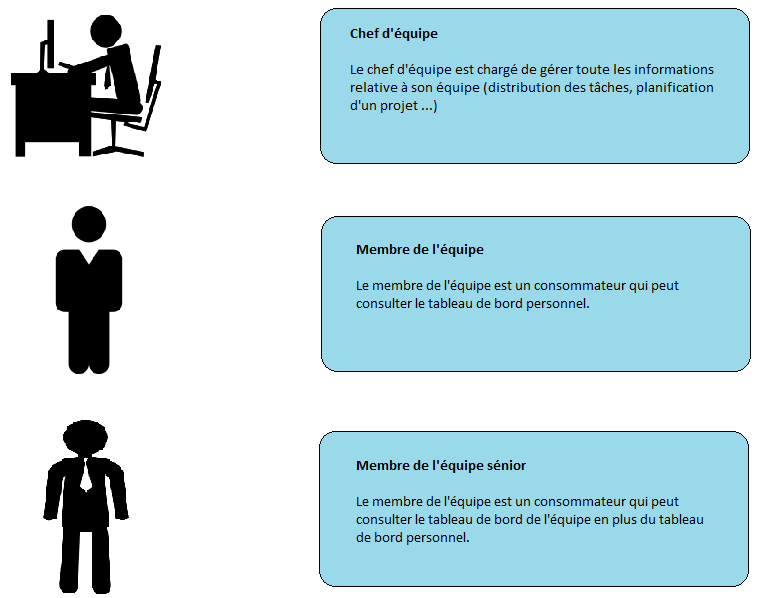
\includegraphics[scale=0.7]{figures/actors.png}
  \caption{Représentation des acteurs}
  \label{code6}
\end{figure}
\subsection{Besoin fonctionnel}
Les besoins fonctionnels représentent ce que le système doit être en mesure d'effectuer. Notre application doit offrir à ces utilisateurs les fonctionnalités suivantes: \\
\begin{itemize}
	\item[$\bullet$] Le membre de l'équipe doit pouvoir:
     \begin{itemize}
     	\item[$\circ$] s'authentifier
        \item[$\circ$] consulter le tableau de bord personnel\\
    \end{itemize}
    \item[$\bullet$] Le membre de l'équipe senior doit pouvoir:
    \begin{itemize}
     	\item[$\circ$] s'authentifier
        \item[$\circ$] consulter les tableaux de bord de l'équipe 
        \item[$\circ$] consulter le tableau de bord personnel\\
    \end{itemize}
	\item[$\bullet$] Le chef d'équipe doit pouvoir:
    \begin{itemize}
    	\item[$\circ$] s'authentifier
        \item[$\circ$] gérer les membres
        \item[$\circ$] gérer les équipes
        \item[$\circ$] consulter les tableaux de bord de l'équipe
        \item[$\circ$] gérer les objectifs des ICP \footnote{Indicateur clé de performance (ICP), en anglais Key Performance Indicator (KPI), est un indicateur mesurable d'aide décisionnelle \cite{ICP}.}
        \item[$\circ$] utiliser la fonctionnalité de planification
     
     
     \end{itemize}
\end{itemize}
\subsection{Besoin non fonctionnel}
Les besoins non fonctionnels peuvent être considérés comme des besoins
fonctionnels spéciaux. Parfois, ils ne sont pas rattachés à un cas d’utilisation
particulier, mais ils caractérisent tout le système (l’architecture, la sécurité, le temps
de réponse, etc.).

Le système doit garantir les besoins opérationnels suivants:\\
\begin{itemize}
	\item[$\bullet$] La sécurité et la confidentialité des données : Les droits d’accès à
l’application doivent être bien attribués aux différents partenaires, afin
d’assurer la sécurité des données.\\
	\item[$\bullet$] Maintenabilité et évolutivité : Le code de l’application doit être bien lisible et
compréhensible pour pouvoir le maintenir facilement et rapidement. En outre,
l’application doit être évolutive afin de répondre aux changements des
besoins fonctionnels.\\
	\item[$\bullet$] Performance: L'application doit garantir un temps de réponse et un temps de traitement réduit.\\
    \item[$\bullet$] Ergonomie: L'application doit avoir une interface conviviale et facile à utiliser et ceci en limitant le nombre des éléments dans l'écran, en utilisant des couleurs qui vont ensemble et en créant des interfaces qui offrent une bonne expérience utilisateur.
\end{itemize}
\section{Diagramme de cas d'utilisation global}
Après avoir identifié les besoins et les acteurs, nous traçons le diagramme de cas d'utilisation global qui sera après la base pour la rédaction du backlog produit.

La figure \ref{code7} présente le diagramme de cas d'utilisation global.
\begin{figure}[H]
  \centering
  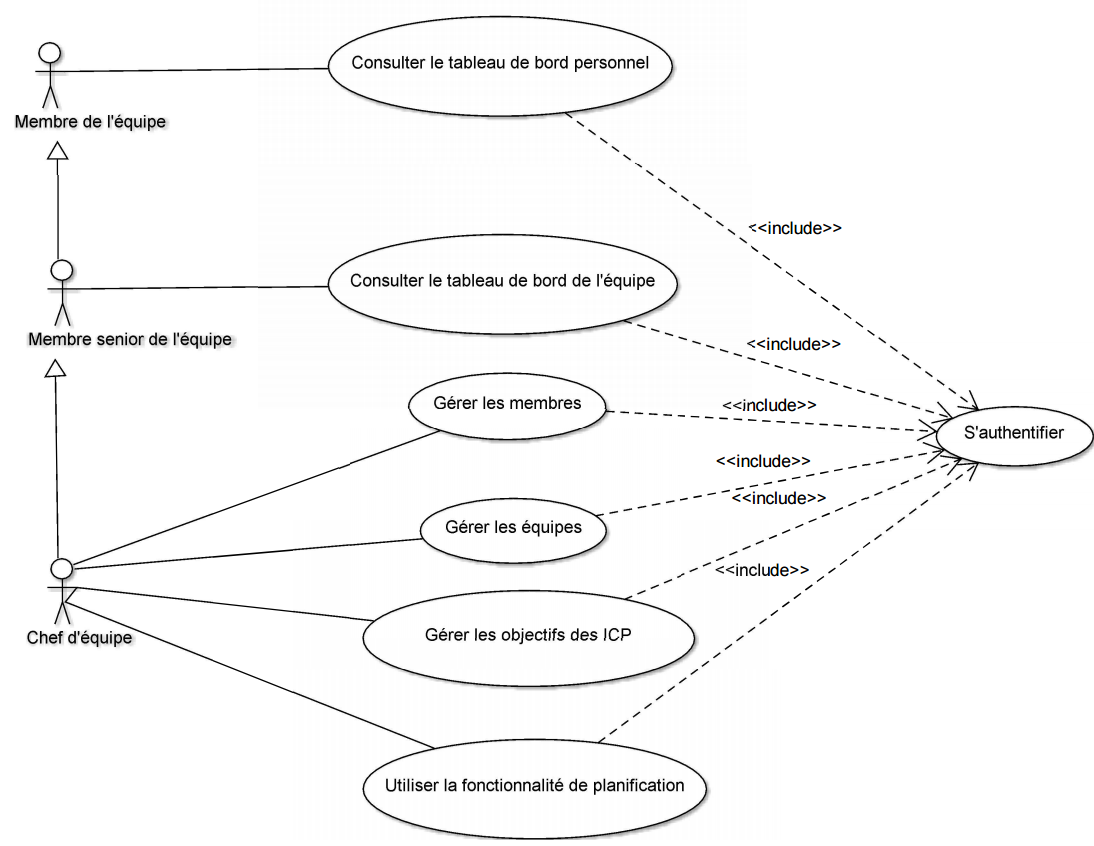
\includegraphics[scale=0.6]{figures/UC_global.png}
  \caption{Diagramme de cas d'utilisation global}
  \label{code7}
\end{figure}
\section{Backlog produit}
Dans Scrum, le backlog produit est la liste des fonctionnalités attendues d'un produit. Il contient donc tous les éléments qui vont nécessiter du travail pour l'équipe. Les éléments y sont classés par priorité ce qui permet de définir l'ordre de réalisation et par complexité ce qui permet de définir la taille d'un backlog sprint.
Nous allons donc présenter les notions de priorité et de complexité. Après nous allons présenter le backlog produit de notre application. Et nous proposerons enfin la planification de release.
\subsection{Notion de priorité}
La priorité représente l'ordre de développement des user stories. Elle permet donc de connaître l'ordre selon lequel les user stories vont être sélectionnées pour être développé dans les backlogs sprint.
Les niveaux de priorité qui vont être utilisé dans notre backlog sont:
\begin{itemize}
	\item[$\bullet$] Élevée: L’exigence est essentielle. Si elle n’est pas faîte le projet échoue.
	\item[$\bullet$] Moyenne: Il s’agit d’une exigence essentielle, qu’il faut faire dans la mesure du possible.
    \item[$\bullet$] Faible: Il s’agit d’une exigence souhaitable. Elle pourrait être faîte dans la mesure où elle n’a pas d’impact sur les autres tâches.
   	\item[$\bullet$] Très faible: Il s’agit d’une exigence "Luxe". Elle ne sera pas faîte cette fois mais plus tard, mais intéressante et à garder pour la prochaine version \cite{Backlog}.
\end{itemize}
\subsection{Notion de complexité}
La notion de complexité(ou Story point) sert à estimer l’effort nécessaire à une équipe pour implémenter une fonctionnalité.
Cette estimation prend en compte l'effort pour le développement, la complexité du développement et le risque \cite{ComplexiteScrum}.

Nous allons utiliser les six premiers nombres de la suite de Fibonacci comme points de complexités dans notre backlog produit (1,2,3,5,8,13) \cite{SuiteFibo}.
\subsection{Backlog produit}
Le tableau \ref{code8} représente le backlog produit de notre application.

\begin{center}
\begin{longtable}{l}
\caption{Backlog produit de l'application} \label{code8} \\
\begin{tabular}{|l|l|l|l|l|l|}
\hline
\textbf{ID} & \textbf{Fonctionnalité} & \textbf{\begin{tabular}[c]{@{}l@{}}ID \\ story\end{tabular}} & \textbf{User Story} & \textbf{Priorité} & \textbf{Complexité} \\ \hline
\multirow{2}{*}{1} & \multirow{2}{*}{s'authentifier} & 1.1 & \begin{tabular}[c]{@{}l@{}}En tant que membre, membre senior \\ ou chef d'équipe, je souhaite pouvoir \\ m'authentifier\end{tabular} & Moyenne & 5 \\ \cline{3-6} 
 &  & 1.2 & \begin{tabular}[c]{@{}l@{}}En tant que membre, membre senior \\ ou chef d'équipe, je souhaite pouvoir \\ modifier mon mot de passe\end{tabular} & Faible & 3 \\ \hline
 
\multirow{3}{*}{2} & \multirow{3}{*}{gérer les équipes} & 2.1 & \begin{tabular}[c]{@{}l@{}}En tant que chef d'équipe, je souhaite \\ pouvoir créer une nouvelle équipe\end{tabular} & Moyenne & 3 \\ \cline{3-6} 
 &  & 2.2 & \begin{tabular}[c]{@{}l@{}}En tant que chef d'équipe, je souhaite \\ pouvoir supprimer une équipe\end{tabular} & Moyenne & 3 \\ \cline{3-6} 
 &  & 2.3 & \begin{tabular}[c]{@{}l@{}}En tant que chef d'équipe, je souhaite \\ pouvoir assigner un chef d'équipe\end{tabular} & Elevé & 3 \\ \hline
 
\multirow{3}{*}{3} & \multirow{3}{*}{gérer les membres} & 3.1 & \begin{tabular}[c]{@{}l@{}}En tant que chef d'équipe, je souhaite\\ pouvoir ajouter un membre dans \\ l'application\end{tabular} & Moyenne & 3 \\ \cline{3-6} 
 &  & 3.2 & \begin{tabular}[c]{@{}l@{}}En tant que chef d'équipe, je souhaite\\ pouvoir supprimer un membre de\\ l'application\end{tabular} & Moyenne & 3 \\ \cline{3-6} 
 &  & 3.3 & \begin{tabular}[c]{@{}l@{}}En tant que chef d'équipe, je souhaite\\ pouvoir modifier un membre de\\ l'application\end{tabular} & Moyenne & 3 \\ \hline
 \end{tabular} \\
 \begin{tabular}{|l|l|l|l|l|l|}
 \hline
 \textbf{ID} & \textbf{Fonctionnalité} & \textbf{\begin{tabular}[c]{@{}l@{}}ID \\ story\end{tabular}} & \textbf{User Story} & \textbf{Priorité} & \textbf{Complexité}
 \\ \hline
4 & \begin{tabular}[c]{@{}l@{}}consulter les \\ tableaux de bord\\ de l'équipe\end{tabular} & 4.1 & \begin{tabular}[c]{@{}l@{}}En tant que membre senior ou chef \\ d'équipe, je souhaite pouvoir consulter \\ le tableaux de bord de l'équipe\end{tabular} & Elevée & 8 \\ \hline
\multirow{2}{*}{5} & \multirow{2}{*}{\begin{tabular}[c]{@{}l@{}}consulter les\\ tableaux de bord\\ personnels\end{tabular}} & 5.1 & \begin{tabular}[c]{@{}l@{}}En tant que membre ou membre senior \\ de l'équipe, je souhaite pouvoir consulter \\ le tableau de bord me représentant\end{tabular} & Faible & 5 \\ \cline{3-6} 
 &  & 5.2 & \begin{tabular}[c]{@{}l@{}}En tant que membre senior ou chef \\ d'équipe, je souhaite pouvoir consulter \\ les tableaux de bord des membres de \\ mon équipe\end{tabular} & Elevée & 13 \\ \hline
6 & \begin{tabular}[c]{@{}l@{}}gérer les objectifs \\ des ICP\end{tabular} & 6.1 & \begin{tabular}[c]{@{}l@{}}En tant que chef d'équipe, je souhaite \\ pouvoir modifier les valeurs des \\ objectifs ICP\end{tabular} & Moyenne & 5 \\ \hline
7 & \begin{tabular}[c]{@{}l@{}}utiliser la \\ fonctionnalité\\ de planification\end{tabular} & 7.1 & \begin{tabular}[c]{@{}l@{}}En tant que chef d'équipe, je souhaite \\ pouvoir saisir les informations relatives \\ à la planification et consulter le résultat \\ obtenu\end{tabular} & Elevée & 13 \\ \hline
\end{tabular}
\end{longtable}
\end{center}

\begin{comment}

\begin{table}[H]
\centering
\caption{Backlog produit de l'application}
\label{code8}
\begin{tabular}{|l|l|l|l|l|l|}
\hline
\textbf{ID} & \textbf{Fonctionnalité} & \textbf{\begin{tabular}[c]{@{}l@{}}ID \\ story\end{tabular}} & \textbf{User Story} & \textbf{Priorité} & \textbf{Complexité} \\ \hline
\multirow{2}{*}{1} & \multirow{2}{*}{s'authentifier} & 1.1 & \begin{tabular}[c]{@{}l@{}}En tant que membre, membre senior \\ ou chef d'équipe, je souhaite pouvoir \\ m'authentifier\end{tabular} & Moyenne & 5 \\ \cline{3-6} 
 &  & 1.2 & \begin{tabular}[c]{@{}l@{}}En tant que membre, membre senior \\ ou chef d'équipe, je souhaite pouvoir \\ modifier mon mot de passe\end{tabular} & Faible & 3 \\ \hline
\multirow{3}{*}{2} & \multirow{3}{*}{gérer les équipes} & 2.1 & \begin{tabular}[c]{@{}l@{}}En tant que chef d'équipe, je souhaite \\ pouvoir créer une nouvelle équipe\end{tabular} & Moyenne & 3 \\ \cline{3-6} 
 &  & 2.2 & \begin{tabular}[c]{@{}l@{}}En tant que chef d'équipe, je souhaite \\ pouvoir supprimer une équipe\end{tabular} & Moyenne & 3 \\ \cline{3-6} 
 &  & 2.3 & \begin{tabular}[c]{@{}l@{}}En tant que chef d'équipe, je souhaite \\ pouvoir assigner un chef d'équipe\end{tabular} & Elevé & 3 \\ \hline
\multirow{3}{*}{3} & \multirow{3}{*}{gérer les membres} & 3.1 & \begin{tabular}[c]{@{}l@{}}En tant que chef d'équipe, je souhaite\\ pouvoir ajouter un membre dans \\ l'application\end{tabular} & Moyenne & 3 \\ \cline{3-6} 
 &  & 3.2 & \begin{tabular}[c]{@{}l@{}}En tant que chef d'équipe, je souhaite\\ pouvoir supprimer un membre de\\ l'application\end{tabular} & Moyenne & 3 \\ \cline{3-6} 
 &  & 3.3 & \begin{tabular}[c]{@{}l@{}}En tant que chef d'équipe, je souhaite\\ pouvoir modifier un membre de\\ l'application\end{tabular} & Moyenne & 3 \\ \hline
4 & \begin{tabular}[c]{@{}l@{}}consulter les \\ tableaux de bord\\ de l'équipe\end{tabular} & 4.1 & \begin{tabular}[c]{@{}l@{}}En tant que membre senior ou chef \\ d'équipe, je souhaite pouvoir consulter \\ le tableaux de bord de l'équipe\end{tabular} & Elevée & 8 \\ \hline
\multirow{2}{*}{5} & \multirow{2}{*}{\begin{tabular}[c]{@{}l@{}}consulter les\\ tableaux de bord\\ personnels\end{tabular}} & 5.1 & \begin{tabular}[c]{@{}l@{}}En tant que membre ou membre senior \\ de l'équipe, je souhaite pouvoir consulter \\ le tableau de bord me représentant\end{tabular} & Faible & 5 \\ \cline{3-6} 
 &  & 5.2 & \begin{tabular}[c]{@{}l@{}}En tant que membre senior ou chef \\ d'équipe, je souhaite pouvoir consulter \\ les tableaux de bord des membres de \\ mon équipe\end{tabular} & Elevée & 13 \\ \hline
6 & \begin{tabular}[c]{@{}l@{}}gérer les objectifs \\ des ICP\end{tabular} & 6.1 & \begin{tabular}[c]{@{}l@{}}En tant que chef d'équipe, je souhaite \\ pouvoir modifier les valeurs des \\ objectifs ICP\end{tabular} & Moyenne & 5 \\ \hline
7 & \begin{tabular}[c]{@{}l@{}}utiliser la \\ fonctionnalité\\ de planification\end{tabular} & 7.1 & \begin{tabular}[c]{@{}l@{}}En tant que chef d'équipe, je souhaite \\ pouvoir saisir les informations relatives \\ à la planification et consulter le résultat \\ obtenu\end{tabular} & Elevée & 13 \\ \hline
\end{tabular}
\end{table}
\end{comment}

\subsection{Prototypage des interfaces}
La figure \ref{code10} présente le prototype de l'interface de la page d'authentification.
\begin{figure}[H]
  \centering
  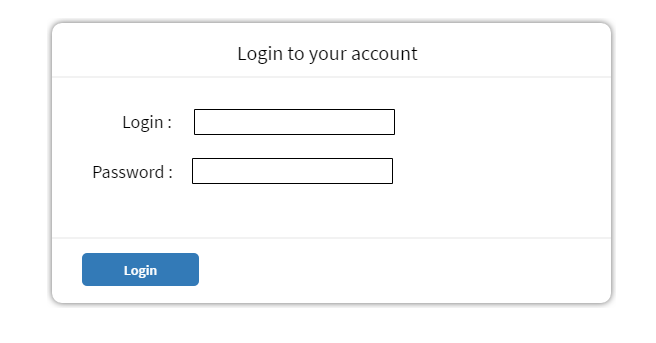
\includegraphics[scale=1]{figures/prototypes/Login_form.PNG}
  \caption{Prototype de la page d'authentification}
  \label{code10}
\end{figure}
La figure \ref{code11} présente le prototype du tableau de bord personnel où nous retrouverons toutes les statistiques concernant l'utilisateur connecté.
\begin{figure}[H]
  \centering
  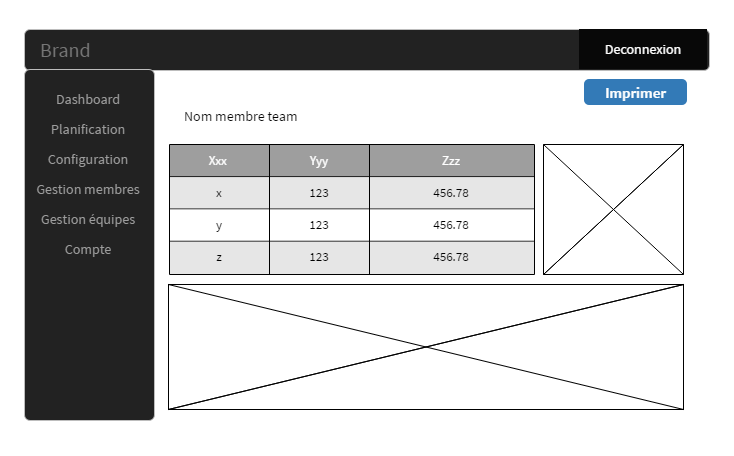
\includegraphics[scale=0.74]{figures/prototypes/Member_dashboard.PNG}
  \caption{Prototype du tableau de bord personnel}
  \label{code11}
\end{figure}
La figure \ref{code12} présente le prototype du tableau de bord de l'équipe ou en retrouve des statistiques qui concernent toute l'équipe.
\begin{figure}[H]
  \centering
  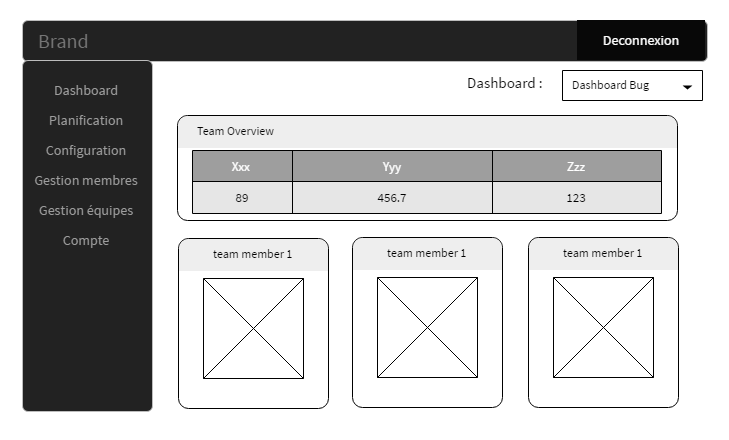
\includegraphics[scale=0.74]{figures/prototypes/Team_dashboard.PNG}
  \caption{Prototype du tableau de bord de l'équipe}
  \label{code12}
\end{figure}
La figure \ref{code13} présente le prototype de l'interface de gestion de compte où l'utilisateur peut changer son mot de passe.
\begin{figure}[H]
  \centering
  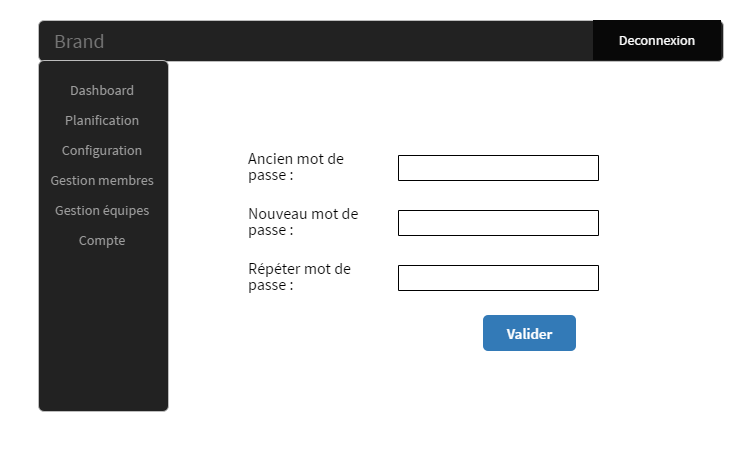
\includegraphics[scale=0.74]{figures/prototypes/Compte.PNG}
  \caption{Prototype de la gestion de compte}
  \label{code13}
\end{figure}
La figure \ref{code14} présente le prototype de l'interface de gestion des objectifs ICP ou l'utilisateur peut modifier les objectifs.
\begin{figure}[H]
  \centering
  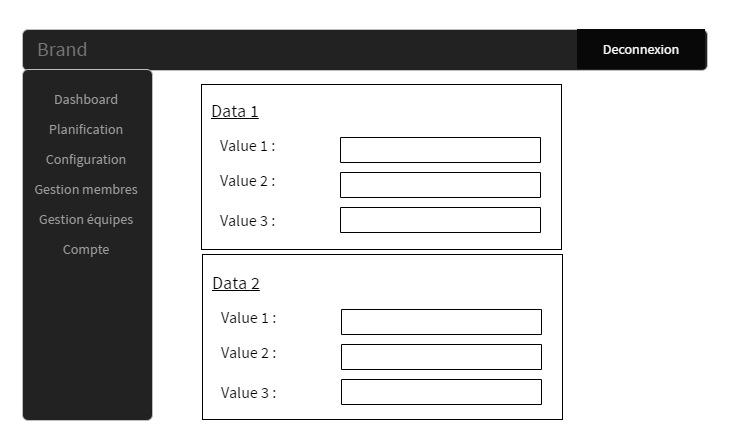
\includegraphics[scale=0.74]{figures/prototypes/Configuration.PNG}
  \caption{Prototype de la gestion des objectifs ICP}
  \label{code14}
\end{figure}
La figure \ref{code15} présente le prototype de l'interface de gestion d'équipe où l'utilisateur peut ajouter, modifier ou supprimer une équipe.
\begin{figure}[H]
  \centering
  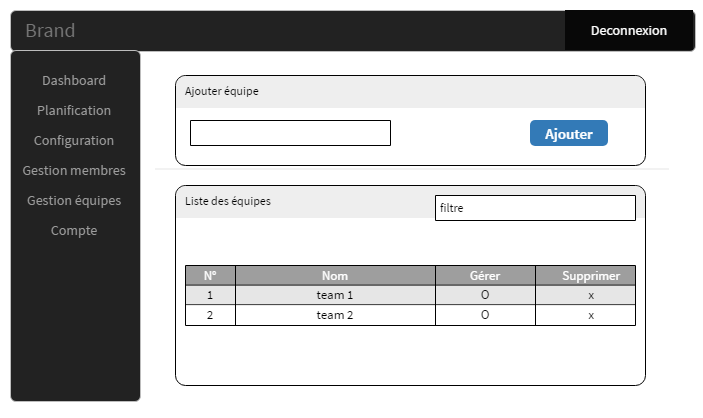
\includegraphics[scale=0.77]{figures/prototypes/Gestion_equipes_1.png}
  \caption{Prototype de la gestion des équipes}
  \label{code15}
\end{figure}
La figure \ref{code16} présente le prototype de l'interface de modification d'équipe où l'utilisateur peut changer le chef d'équipe ou enlever un utilisateur de cette dernière.
\begin{figure}[H]
  \centering
  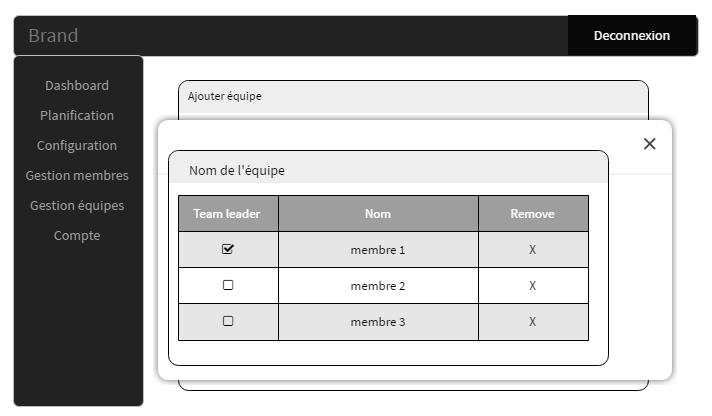
\includegraphics[scale=0.77]{figures/prototypes/Gestion_equipes_2.png}
  \caption{Prototype de la modification d'une équipe}
  \label{code16}
\end{figure}
La figure \ref{code17} présente le prototype de l'interface de gestion des membres où l'utilisateur peut ajouter, modifier ou supprimer un utilisateur de l'application.
\begin{figure}[H]
  \centering
  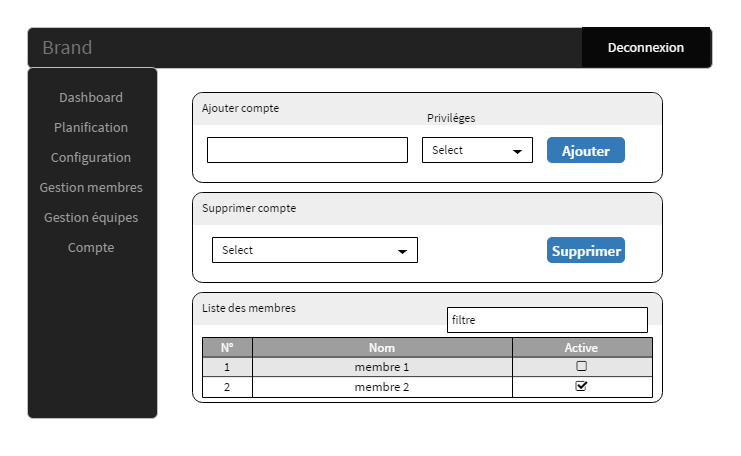
\includegraphics[scale=0.74]{figures/prototypes/Gestion_membres.PNG}
  \caption{Prototype de la gestion des membres}
  \label{code17}
\end{figure}
La figure \ref{code18} présente le prototype de l'interface de planification de tâche.
\begin{figure}[H]
  \centering
  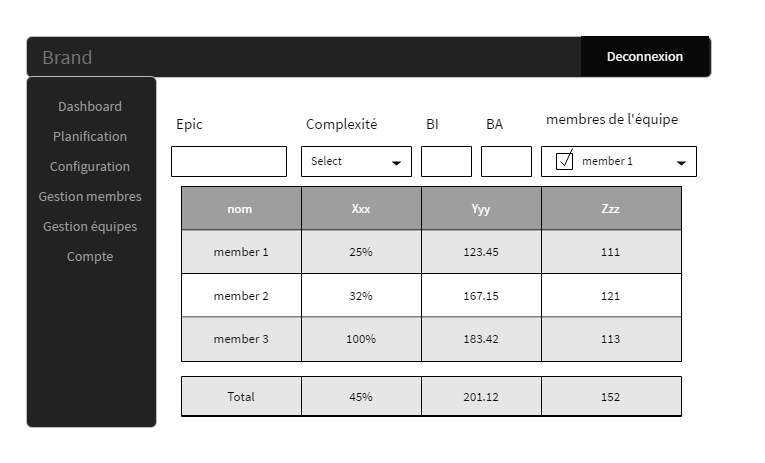
\includegraphics[scale=0.74]{figures/prototypes/Planification.PNG}
  \caption{Prototype de la planification}
  \label{code18}
\end{figure}

\section{Planification de release}
La planification de release est conçu pour décomposer le projet en plusieurs sprints de durée fixe. Pour pouvoir le faire, il faut estimer la complexité totale de user stories qui peuvent être réalisés dans une durée fixe du sprint. Cette valeur estimée s'appelle la vélocité \cite{Planning_sprint} \cite{Estimation_planification_Agile}. La durée d'un sprint pour notre projet va être fixé à 4 semaines et nous avons conclu que la vélocité sera égale à 21. La figure \ref{code19} représente la planification de release pour notre projet.

\begin{figure}[H]
\centering
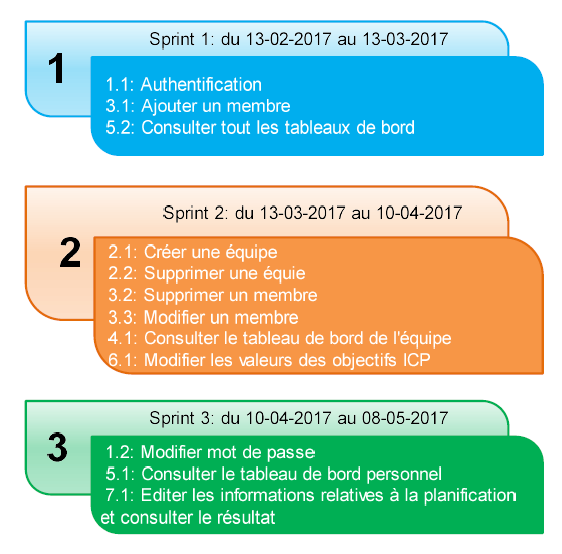
\includegraphics[scale=0.9]{figures/sprints_release_planification.png}
\caption{Planification de release de notre projet}
\label{code19}
\end{figure}
\section{Conclusion}
Dans ce chapitre nous avons présenté les besoins fonctionnels, les besoins non fonctionnels et les acteurs de notre application. Puis, nous avons présenté le diagramme de cas d'utilisation initiale. Après, nous avons défini la notion de priorité et celle de complexité. Ensuite, nous avons présenté le product backlog. Et enfin, nous avons présenté le prototypage et la planification de release qu'on va suivre tout au long de notre projet. Dans le prochain chapitre nous allons détailler nos choix architecturaux ainsi que l'environnement de travail matériel et logiciel.
\chapter{Conception et réalisation de l'application}
\section{Introduction}
Dans ce chapitre, nous allons présenter l'environnement de travail et les choix architecturaux. En premier lieu, nous parlerons de l'environnement matériel et logiciel. Après, nous proposerons nos choix architecturaux.
\section{Environnement de travail}
Cette section va être dédiée à la présentation de l'environnement de travail que ce soit matériel ou logiciel.
\subsection{Environnement matériel}
Le tableau \ref{code20} présente les caractéristiques techniques de la machine utilisé.
\begin{table}[H]
\centering
\caption{Caractéristiques techniques de la machine}
\label{code20}
\begin{tabular}{|l|l|}
\hline
\textbf{Constructeur} & Dell Inc. \\
\hline
\textbf{Processeur} & Intel(R) Core(TM) i3-2100 CPU @ 3.10GHz \\ \hline
\textbf{RAM} & 8.0 GO \\ \hline
\textbf{Disque dur} & 500.0 GO \\ \hline
\textbf{Système d'exploitation} & Microsoft Windows 10 Entreprise (x64) \\ \hline
\end{tabular}
\end{table}
\subsection{Environnement logiciel}
Dans cette partie, nous allons présenter les logiciels utilisés en plus des technologies.
\subsubsection{Eclipse}
\noindent\begin{minipage}{0.69\textwidth}
Eclipse est un environnement de développement intégré qui est open source. Cet outil a été utilisé pour développer la partie back-office \footnotemark de l'application qui est en Java.
\end{minipage}
\footnotetext{Back-office désigne les applications qui ne sont pas accessibles au client final}
\begin{minipage}{0.3\textwidth}
\begin{figure}[H]
  \centering
  
\includegraphics[scale=0.6]{figures/logo/eclipse.png}
  \caption{Logo Eclipse}
  \label{code21}
\end{figure}
\end{minipage}
\subsubsection{Sublime Text 3}
\noindent\begin{minipage}{0.69\textwidth}
Sublime Text 3 est un éditeur de texte qui facilite la saisie de code grâce à son auto-complétion, aux différents raccourcis et à la coloration de syntaxe. Cet outil a été utilisé pour développer la partie front-office \footnotemark de l'application qui est en Javascript, HTML et CSS.
\end{minipage}
\footnotetext{Front-office désigne les applications accessibles au client final}
\begin{minipage}{0.3\textwidth}
\begin{figure}[H]
  \centering
  
\includegraphics[scale=0.25]{figures/logo/Sublime_Text_3.png}
  \caption{Logo Sublime Text}
  \label{code22}
\end{figure}
\end{minipage}
\subsubsection{Oracle SQL Developer}
\noindent\begin{minipage}{0.69\textwidth}
Oracle SQL Developer est environnement de développement intégré permettant d'interroger les bases de données Oracle grâce au langage SQL. Cet outil a été utilisé pour consulter la base de données distante de l'application Jira en plus de la base de données de notre application.
\end{minipage}
\begin{minipage}{0.3\textwidth}
\begin{figure}[H]
  \centering
  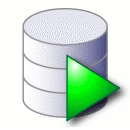
\includegraphics[scale=0.5]{figures/logo/orclsqldev3.jpg}
  \caption{Logo Oracle SQL Developer}
  \label{code23}
\end{figure}
\end{minipage}
\subsubsection{Edraw Max}
\noindent\begin{minipage}{0.69\textwidth}
Edraw Max est un logiciel permettant de créer des diagrammes de toutes sortes. Ce logiciel a été utilisé pour la création de l'organigramme de la société.
\end{minipage}
\begin{minipage}{0.3\textwidth}
\begin{figure}[H]
  \centering
  
\includegraphics[scale=0.25]{figures/logo/edraw_max.png}
  \caption{Logo Edraw max}
  \label{code24}
\end{figure}
\end{minipage}
\subsubsection{Enterprise Architect}
\noindent\begin{minipage}{0.69\textwidth}
Enterprise Architect est un logiciel permettant de créer des diagrammes UML. Ce logiciel a été utilisé pour la conception de notre application afin de créer les diagrammes UML utilisés dans le rapport.
\end{minipage}
\begin{minipage}{0.3\textwidth}
\begin{figure}[H]
  \centering
  
\includegraphics[scale=0.3]{figures/logo/enterprisearchitect.png}
  \caption{Logo Enterprise Architect}
  \label{code25}
\end{figure}
\end{minipage}
\subsubsection{Google Chrome}
\noindent\begin{minipage}{0.69\textwidth}
Google Chrome est un navigateur web disposant d'une console permettant de debug le code de notre application front-office. Cet outil a été utilisé pour la visualisation de l'application web.
\end{minipage}
\begin{minipage}{0.3\textwidth}
\begin{figure}[H]
  \centering
  
\includegraphics[scale=0.2]{figures/logo/chrome.png}
  \caption{Logo Google Chrome}
  \label{code26}
\end{figure}
\end{minipage}
\subsubsection{Postman}
\noindent\begin{minipage}{0.69\textwidth}
Postman est une application permettant de tester les services web. Cette application a été utilisé pour tester tous les services web de notre application back-office.
\end{minipage}
\begin{minipage}{0.3\textwidth}
\begin{figure}[H]
  \centering
  
\includegraphics[scale=0.12]{figures/logo/postman.png}
  \caption{Logo Postman}
  \label{code27}
\end{figure}
\end{minipage}
\subsubsection{Overleaf}
\noindent\begin{minipage}{0.69\textwidth}
Overleaf est un éditeur de rapport Latex en ligne. Il dispose d'outil de gestion de version en plus de sa facilité d'utilisation. Cet outil a été utilisé pour éditer le rapport de notre projet de fin d'études.
\end{minipage}
\begin{minipage}{0.3\textwidth}
\begin{figure}[H]
  \centering
  
\includegraphics[scale=1]{figures/logo/overleaf.png}
  \caption{Logo Overleaf}
  \label{code28}
\end{figure}
\end{minipage}
\subsubsection{Sharelatex}
\noindent\begin{minipage}{0.69\textwidth}
Sharelatex est aussi un éditeur de rapport Latex en ligne. En plus de sa facilité d'utilisation, ce dernier n'a pas de limitations si vous allez l'utiliser sans collaborateurs. Cet outil a été utilisé pour éditer le rapport de notre projet de fin d'études.
\end{minipage}
\begin{minipage}{0.3\textwidth}
\begin{figure}[H]
  \centering
  
\includegraphics[scale=0.25]{figures/logo/sharelatex.jpg}
  \caption{Logo Sharelatex}
  \label{code52}
\end{figure}
\end{minipage}
\subsubsection{Trello}
\noindent\begin{minipage}{0.69\textwidth}
Trello est un outil de gestion de projet en ligne. Nous l'avons utilisé pour gérer les sprints de notre projet.
\end{minipage}
\begin{minipage}{0.3\textwidth}
\begin{figure}[H]
  \centering
  
\includegraphics[scale=0.3]{figures/logo/trello.png}
  \caption{Logo Trello}
  \label{code29}
\end{figure}
\end{minipage}
\subsubsection{Ollert}
\noindent\begin{minipage}{0.69\textwidth}
Ollert est un outil de génération de rapports sur l'avancement d'un projet géré par Trello. Cet outil a été utilisé pour visualiser notre avancement tout au long du projet.
\end{minipage}
\begin{minipage}{0.3\textwidth}
\begin{figure}[H]
  \centering
  
\includegraphics[scale=0.2]{figures/logo/ollert.png}
  \caption{Logo Ollert}
  \label{code30}
\end{figure}
\end{minipage}
\subsubsection{DB Designer}
\noindent\begin{minipage}{0.69\textwidth}
DB Designer est un outil de création d'un schéma de base de données en ligne. Cet outil permet d'exporter le schéma sous format SQL. Nous avons utilisé ce dernier pour pouvoir créer le schéma de base de données de notre application afin de pouvoir en discuter lors des réunions hebdomadaires.
\end{minipage}
\begin{minipage}{0.3\textwidth}
\begin{figure}[H]
  \centering
  
\includegraphics[scale=1]{figures/logo/db_designer.png}
  \caption{Logo DB Designer}
  \label{code31}
\end{figure}
\end{minipage}
\subsubsection{Jira}
\noindent\begin{minipage}{0.69\textwidth}
Jira est un outil de gestion de projet piloté par Scrum ou Kanban \footnotemark. Cet outil est utilisé dans la société pour piloter les projets et sa base de données contient des informations sur les employés de cette dernière. Nous avons utilisé Jira pour pouvoir en extraire les données sur les employés afin de calculer les indicateurs de performance.
\end{minipage}
\footnotetext{C'est une méthode de travail japonaise connu pour son efficacité dans la gestion de projet}
\begin{minipage}{0.3\textwidth}
\begin{figure}[H]
  \centering
  
\includegraphics[scale=0.3]{figures/logo/jira.jpg}
  \caption{Logo Jira}
  \label{code32}
\end{figure}
\end{minipage}
\subsubsection{Apache Tomcat}
\noindent\begin{minipage}{0.69\textwidth}
Apache Tomcat est un serveur HTTP et conteneur web libre de servlet \cite{Tomcat}. Cet outil a été utilisé pour héberger notre application back-office.
\end{minipage}
\begin{minipage}{0.3\textwidth}
\begin{figure}[H]
  \centering
  
\includegraphics[scale=0.17]{figures/logo/tomcat.png}
  \caption{Logo Apache Tomcat}
  \label{code33}
\end{figure}
\end{minipage}
\subsubsection{Yeoman}
\noindent\begin{minipage}{0.69\textwidth}
Yeoman est un générateur de code utilisé pour générer des projets web. Cet outil a été utilisé pour générer le squelette initial de notre application web en plus des composants de cette dernière.
\end{minipage}
\begin{minipage}{0.3\textwidth}
\begin{figure}[H]
  \centering
  
\includegraphics[scale=0.17]{figures/logo/yeoman.png}
  \caption{Logo Yeoman}
  \label{code34}
\end{figure}
\end{minipage}
\subsubsection{Dozer}
\noindent\begin{minipage}{0.69\textwidth}
Dozer est un outil de mise en correspondance des données en Java / JEE. Cet outil a été utilisé pour mettre en correspondance les modèles et les entités.
\end{minipage}
\begin{minipage}{0.3\textwidth}
\begin{figure}[H]
  \centering
  
\includegraphics[scale=0.38]{figures/logo/dozer.png}
  \caption{Logo Dozer}
  \label{code35}
\end{figure}
\end{minipage}
\subsubsection{NodeJs}
\noindent\begin{minipage}{0.69\textwidth}
NodeJs est un runtime Javascript permettant d’exécuter du code Javascript côté serveur. Cet outil dispose aussi d'un manager de paquetage Javascript Open Source appelé Npm. Cet outil a été utilisé pour installer différents paquetages pour notre projet front-office.
\end{minipage}
\begin{minipage}{0.3\textwidth}
\begin{figure}[H]
  \centering
  
\includegraphics[scale=0.12]{figures/logo/nodejs.jpg}
  \caption{Logo NodeJS}
  \label{code36}
\end{figure}
\end{minipage}
\subsubsection{Bower}
\noindent\begin{minipage}{0.69\textwidth}
Bower est un manager de paquetage comme Npm. Cet outil a aussi été utilisé pour installer différents paquetages pour notre projet front-office.
\end{minipage}
\begin{minipage}{0.3\textwidth}
\begin{figure}[H]
  \centering
  
\includegraphics[scale=0.17]{figures/logo/bower.png}
  \caption{Logo Bower}
  \label{code37}
\end{figure}
\end{minipage}
\subsubsection{Grunt}
\noindent\begin{minipage}{0.69\textwidth}
Grunt est un outil d'automatisation de code Javascript. Cet outil a été utilisé comme serveur http pour héberger notre application front-office et pour gérer le changement de code.
\end{minipage}
\begin{minipage}{0.3\textwidth}
\begin{figure}[H]
  \centering
  
\includegraphics[scale=0.25]{figures/logo/grunt.png}
  \caption{Logo Grunt}
  \label{code38}
\end{figure}
\end{minipage}
\subsubsection{Maven}
\noindent\begin{minipage}{0.69\textwidth}
Maven est un moteur de production pour les applications Java / JEE. Cet outil a été utilisé pour gérer les dépendances du projet en plus de la génération de codes.
\end{minipage}
\begin{minipage}{0.3\textwidth}
\begin{figure}[H]
  \centering
  
\includegraphics[scale=0.4]{figures/logo/maven.png}
  \caption{Logo Maven}
  \label{code39}
\end{figure}
\end{minipage}
\subsubsection{Hibernate}
\noindent\begin{minipage}{0.69\textwidth}
Hibernate est un ORM \footnotemark servant à la gestion de persistance de la base de données relationnelle. Cet outil a été utilisé pour gérer la base de données de notre application back-office.
\end{minipage}
\footnotetext{Object Relationship Mapping ou en français Mapping objet relationnel est un outil permettant de gérer la persistance des données entre l'application et la base de données relationnelle}
\begin{minipage}{0.3\textwidth}
\begin{figure}[H]
  \centering
  
\includegraphics[scale=0.35]{figures/logo/hibernate.png}
  \caption{Logo Hibernate}
  \label{code40}
\end{figure}
\end{minipage}
\subsubsection{Spring}
\noindent\begin{minipage}{0.69\textwidth}
Spring est un framework Java / JEE conçu pour faciliter le développement d'applications. Ce framework a plusieurs avantages tels que la facilité d'utilisation ou son architecture robuste et facile à comprendre. Ce framework a été utilisé pour développer notre application back-office.
\end{minipage}
\begin{minipage}{0.3\textwidth}
\begin{figure}[H]
  \centering
  
\includegraphics[scale=0.35]{figures/logo/spring.png}
  \caption{Logo Spring}
  \label{code41}
\end{figure}
\end{minipage}
\subsubsection{AngularJS}
\noindent\begin{minipage}{0.69\textwidth}
AngularJS est un framework MVC \footnotemark Javascript conçu pour développer des applications web. Ce framework a été utilisé pour développer notre application front-office.
\end{minipage}
\footnotetext{Model-View-Controller ou en français modéle, vue et contrôleur est une architecture logicielle populaire pour les applications web}
\begin{minipage}{0.3\textwidth}
\begin{figure}[H]
  \centering
  
\includegraphics[scale=0.5]{figures/logo/angularjs.png}
  \caption{Logo AngularJS}
  \label{code42}
\end{figure}
\end{minipage}
\subsubsection{Java}
\noindent\begin{minipage}{0.69\textwidth}
Java est un langage de programmation orienté objet qui permet de développer une application indépendante des architectures logicielles \cite{Java}. Ce langage a été utilisé pour développer l'application back-office.
\end{minipage}
\begin{minipage}{0.3\textwidth}
\begin{figure}[H]
  \centering
  
\includegraphics[scale=0.15]{figures/logo/java.png}
  \caption{Logo Java}
  \label{code43}
\end{figure}
\end{minipage}
\subsubsection{Javascript}
\noindent\begin{minipage}{0.69\textwidth}
Javascript est un langage de programmation conçu pour rendre les pages web dynamiques. Ce langage a été utilisé pour développer notre application front-office.
\end{minipage}
\begin{minipage}{0.3\textwidth}
\begin{figure}[H]
  \centering
  
\includegraphics[scale=0.35]{figures/logo/javascript.png}
  \caption{Logo Javascript}
  \label{code44}
\end{figure}
\end{minipage}
\subsubsection{HTML5}
\noindent\begin{minipage}{0.69\textwidth}
HTML5 est un langage de balisage qui permet de concevoir une interface IHM \footnotemark d'un site web. Ce langage a été utilisé pour créer les interfaces graphiques de notre application front-office.
\end{minipage}
\footnotetext{Interface Homme Machine}
\begin{minipage}{0.3\textwidth}
\begin{figure}[H]
  \centering
  
\includegraphics[scale=0.13]{figures/logo/html.png}
  \caption{Logo HTML5}
  \label{code45}
\end{figure}
\end{minipage}
\subsubsection{CSS3}
\noindent\begin{minipage}{0.69\textwidth}
CSS3 est un langage qui permet de décrire le style d'un document HTML. Ce dernier a été utilisé pour définir le style de notre application.
\end{minipage}
\begin{minipage}{0.3\textwidth}
\begin{figure}[H]
  \centering
  
\includegraphics[scale=0.35]{figures/logo/css.png}
  \caption{Logo CSS3}
  \label{code46}
\end{figure}
\end{minipage}
\subsubsection{JQuery}
\noindent\begin{minipage}{0.69\textwidth}
JQuery est un framework Javascript qui permet de simplifier le développement en Javascript. Ce framework a été utilisé pour développer notre application front-office.
\end{minipage}
\begin{minipage}{0.3\textwidth}
\begin{figure}[H]
  \centering
  
\includegraphics[scale=0.35]{figures/logo/jquery.png}
  \caption{Logo Jquery}
  \label{code47}
\end{figure}
\end{minipage}
\subsubsection{Ajax}
\noindent\begin{minipage}{0.69\textwidth}
Ajax est une bibliothèque Javascript qui permet de modifier une partie d'une page web sans la recharger. Cette dernière a été utilisé pour consommer les services web côté client fourni par notre application back-office.
\end{minipage}
\begin{minipage}{0.3\textwidth}
\begin{figure}[H]
  \centering
  
\includegraphics[scale=0.4]{figures/logo/ajax.jpg}
  \caption{Logo Ajax}
  \label{code48}
\end{figure}
\end{minipage}
\subsubsection{Bootstrap}
\noindent\begin{minipage}{0.69\textwidth}
Bootstrap est un framework Html/Css/Javascript qui fournit à son utilisateur un ensemble d'outils pour créer des pages web dynamiques et ergonomiques.
\end{minipage}
\begin{minipage}{0.3\textwidth}
\begin{figure}[H]
  \centering
  
\includegraphics[scale=0.15]{figures/logo/bootstrap.jpg}
  \caption{Logo Bootstrap}
  \label{code49}
\end{figure}
\end{minipage}
\subsubsection{Oracle Database}
\noindent\begin{minipage}{0.69\textwidth}
Oracle Database est un système de gestion de base de données (SGBD) pour le stockage des données de l'application. Il a été utilisé pour stockage des données de notre application en plus de la consultation des données déjà stocké dans la base de données Jira (externe).
\end{minipage}
\begin{minipage}{0.3\textwidth}
\begin{figure}[H]
  \centering
  \includegraphics[scale=0.4]{figures/logo/oracle_database.png}
  \caption{Logo Oracle Database}
  \label{code50}
\end{figure}
\end{minipage}
\subsubsection{SQL}
\noindent\begin{minipage}{0.69\textwidth}
SQL est un langage de requêtes utilisé pour communiquer avec les SGBD. Ce dernier a été utilisé pour interagir avec nos bases de données.
\end{minipage}
\begin{minipage}{0.3\textwidth}
\begin{figure}[H]
  \centering
  \includegraphics[scale=0.4]{figures/logo/sql.png}
  \caption{Logo SQL}
  \label{code51}
\end{figure}
\end{minipage}
\subsubsection{Mockflow}
\noindent\begin{minipage}{0.69\textwidth}
Mockflow est un outil de dessin de maquette en ligne. Il a été utilisé pour réaliser les prototypes des interfaces.
\end{minipage}
\begin{minipage}{0.3\textwidth}
\begin{figure}[H]
  \centering
  \includegraphics[scale=0.2]{figures/logo/mockflow.png}
  \caption{Logo Mockflow}
  \label{code53}
\end{figure}
\end{minipage}
\section{Choix architecturaux}
Cette section va être dédiée à la présentation du pattern et style architecturaux qui ont été utilisé dans notre application.
\subsection{Style architectural}
Un style architectural est une modélisation du système et sa répartition. Ce dernier est conçu pour aider à avoir un aperçu du système.
Notre système va être décomposé en plusieurs parties:\\
\begin{itemize}
    \item[$\bullet$] Deux couches d'accès aux données: La première pour accéder aux données que nous utiliserons pour calculer les ICP, et la seconde est pour gérer les données de notre application comme les données des utilisateurs ou les données en relation avec les équipes.
    \item[$\bullet$] Deux couches métiers: La première va servir d'intermédiaire entre les couches d'accès aux données et la couche métier de contrôle, et la seconde va servir de contrôleur des vues de la couche présentation.
    \item[$\bullet$] Une couche présentation qui va s'occuper de l'interface graphique.\\
\end{itemize}
Nous avons choisi donc d'utiliser le style architectural N-tiers. La figure \ref{code54} représente la modélisation de notre système.
\begin{figure}[H]
  \centering
  \includegraphics[scale=0.8]{figures/style_architecture.png}
  \caption{Modélisation du système}
  \label{code54}
\end{figure}
\subsection{Pattern architectural}
Un pattern architectural est modèle de référence qui sert à concevoir un système d'information en donnant les sous-systèmes qui le composent , les relations et un ensemble de règles à suivre afin d'organiser les relations entre ces derniers \cite{PatternArchitectural}.
Notre système suit deux patterns architecturaux:\\
\begin{itemize}
    \item[$\bullet$] L’inversion de contrôle (IoC) qui est un pattern architectural qui donne le contrôle du flux d'exécution au framework utilisé. Il existe plusieurs représentations de l'IoC, le framework Spring utilise l'injection de dépendance qui permet de découpler les dépendances entre les objets du projet \cite{IoC}.
    \item[$\bullet$] Modèle - vue - vue modèle (MVVM) qui est un pattern architectural qui permet de séparer entre le modèle et la vue en mettant une vue-modèle comme intermédiaire entre les deux. Ce dernier joue le rôle de convertisseur entre la vue et le modèle. AngularJS utilisent ce qu'on appelle liaison de données (data-binding en anglais) qui permet de modifier la vue si le modèle change et vis versa \cite{MVVM}.\\
\end{itemize}
La figure \ref{code55} présente le pattern architectural de notre application.
\begin{figure}[H]
  \centering
  \includegraphics[scale=0.65]{figures/pattern_diagram.png}
  \caption{Pattern Architectural}
  \label{code55}
\end{figure}
\section{Conclusion}
Dans ce chapitre nous avons présenté l'environnement matériel et logiciel de notre application. Ensuite nous avons détaillé notre style architectural. Et enfin, nous avons présenté le pattern architectural de notre projet. Dans le prochain chapitre, nous allons présenter l'organisation de nos sprints.
\chapter{Organisation des sprints}
\section{Introduction}
Dans ce chapitre, nous allons présenter les sprints de notre projet. En premier lieu, nous allons spécifier le planning pour chaque sprint. Après, nous présenterons la modélisation statique et dynamique. Ensuite, nous allons détailler le développement du sprint. Et enfin, nous allons présenter le test, la revue du sprint et la rétrospective.

\section{Sprint 1: Tableaux de bords (du 13-02-2017 au 13-03-2017)}
Dans cette section, nous allons détailler la réalisation du sprint 1. En premier lieu, nous allons présenter la planification du sprint en présentant le but du sprint et le backlog sprint. Ensuite nous allons spécifier la modélisation statique et la modélisation dynamique. Puis, nous allons présenter le développement du sprint sous forme de capture d'écrans. Et nous finirons, enfin, avec le test, la revue et la rétrospective du sprint. 

\subsection{Sprint planning}
%But du sprint + backlog sprint%
Le but de ce sprint est de créer des tableaux de bords fonctionnels qui utilisent des données de notre base de données Jira. De ce fait, nous proposons le backlog sprint qui est représenté dans la table \ref{code56}.

\begin{longtable}{l}
\caption{Backlog du sprint1: "Tableaux de bords"} \label{code56} \\
\begin{tabular}{|c|l|l|l|}
\hline
\multicolumn{1}{|l|}{\textbf{User storyID}} & \textbf{User Story} & \textbf{Tâche ID} & \textbf{Tâche} \\ \hline
\multirow{3}{*}{1.1} & \multirow{3}{*}{\begin{tabular}[c]{@{}l@{}}En tant que membre, membre \\ senior ou chef d'équipe, je \\ souhaite pouvoir m'authentifier.\end{tabular}} & 1.1.1 & \begin{tabular}[c]{@{}l@{}}Réaliserles diagrammes UML \\ de la fonctionnalité \\ "s'authentifier".\end{tabular} \\ \cline{3-4} 
 &  & 1.1.2 & \begin{tabular}[c]{@{}l@{}}Développer la fonctionnalité \\ "s'authentifier".\end{tabular} \\ \cline{3-4} 
 &  & 1.1.3 & \begin{tabular}[c]{@{}l@{}}Tester la fonctionnalité \\ "s'authentifier".\end{tabular} \\ \hline
 \end{tabular} \\
\begin{tabular}{|c|l|l|l|}
\hline
\multicolumn{1}{|l|}{\textbf{User story ID}} & \textbf{User Story} & \textbf{Tâche ID} & \textbf{Tâche} \\ \hline
\multirow{3}{*}{3.1} & \multirow{3}{*}{\begin{tabular}[c]{@{}l@{}}En tant que chef d’équipe, \\ je souhaite pouvoir ajouter \\ un membre dans l’application.\end{tabular}} & 3.1.1 & \begin{tabular}[c]{@{}l@{}}Réaliser les diagrammes UML \\ de la fonctionnalité "Ajouter un \\ membre".\end{tabular} \\ \cline{3-4} 
 &  & 3.1.2 & \begin{tabular}[c]{@{}l@{}}Développer la fonctionnalité \\"Ajouter un membre".\end{tabular} \\ \cline{3-4} 
 &  & 3.1.3 & \begin{tabular}[c]{@{}l@{}}Tester la fonctionnalité "Ajouter \\un membre".\end{tabular} \\ \hline
\multirow{3}{*}{5.2} & \multirow{3}{*}{\begin{tabular}[c]{@{}l@{}}En tant que membre senior \\ ou chefd’équipe, je souhaite \\ pouvoir consulter les tableaux \\ de bord des membres de mon \\ équipe.\end{tabular}} & 5.2.1 & \begin{tabular}[c]{@{}l@{}}Réaliser les diagrammes UML\\ de la fonctionnalité "Consulter \\ tout les tableaux de bord".\end{tabular} \\ \cline{3-4} 
\multicolumn{1}{|l|}{} &  & 5.2.2 & \begin{tabular}[c]{@{}l@{}}Développer la fonctionnalité \\"Consulter tout les tableaux \\de bord".\end{tabular} \\ \cline{3-4} 
\multicolumn{1}{|l|}{} &  & 5.2.3 & \begin{tabular}[c]{@{}l@{}}Tester la fonctionnalité \\"Consulter tout les tableaux \\de bord".\end{tabular} \\ \hline
\end{tabular}
\end{longtable}

\subsection{Modélisation statique}
%Diagramme de classes%
La modélisation statique permet d'avoir une idée sur les objets et les relations entre ces derniers. Nous présentons donc les diagrammes de classes d'analyse pour chaque fonctionnalité.

\subsubsection{S'authentifier}
La figure \ref{code60} représente le diagramme de classes d'analyse de la fonctionnalité "s'authentifier".
\begin{figure}[H]
  \centering
 \includegraphics[scale=0.69]{figures/diagrams/class/authentification_class_diag.png}
 \caption{Diagramme de classes d'analyse de la fonctionnalité "s'authentifier"}
 \label{code60}
\end{figure}

\subsubsection{Ajouter un membre}
La figure \ref{code61} représente le diagramme de classes d'analyse de la fonctionnalité "ajouter un membre".
\begin{figure}[H]
  \centering
 \includegraphics[scale=0.69]{figures/diagrams/class/addmember_class_diag.png}
 \caption{Diagramme de classes d'analyse de la fonctionnalité "Ajouter un membre"}
 \label{code61}
\end{figure}

\subsubsection{Consulter tout les tableaux de bord}
La figure \ref{code62} représente le diagramme de classes d'analyse de la fonctionnalité "Consulter tout les tableaux de bord".
\begin{figure}[H]
  \centering
 \includegraphics[scale=0.69]{figures/diagrams/class/consulteralldashboard_class_diag.png}
 \caption{Diagramme de classes d'analyse de la fonctionnalité "Consulter tout les tableaux de bord"}
 \label{code62}
\end{figure}

\newpage
\subsection{Modélisation dynamique}
%Diagramme de séquences détaillé ou état transition%
La modélisation dynamique permet d'avoir une idée sur le flux d'exécution de notre application. Nous présentons donc les diagrammes de séquences pour chaque fonctionnalité.

\subsubsection{S'authentifier}
Pour s'authentifier, le membre de l'équipe saisie son nom d'utilisateur et son mot de passe. Puis, il valide par le bouton login. Si la combinaison est incorrecte, un message d'erreur apparaît. Sinon, l'utilisateur est redirigé vers la page d'accueil.
La figure \ref{code57} représente le diagramme de séquence de la fonctionnalité "s'authentifier".
\begin{figure}[H]
  \centering
  \includegraphics[scale=0.7]{figures/diagrams/sequence/authentification_seq_diag.png}
  \caption{Diagramme de séquence de la fonctionnalité "S'authentifier"}
  \label{code57}
\end{figure}

\subsubsection{Ajouter un membre}
Pour ajouter un membre, le chef d'équipe doit sélectionner le nom du membre à ajouter. Puis, il valide par le bouton ajouter.
La figure \ref{code58} représente le diagramme de séquence de la fonctionnalité "ajouter un membre".
\begin{figure}[H]
  \centering
 \includegraphics[scale=0.7]{figures/diagrams/sequence/ajoutermembre_seq_diag.png}
 \caption{Diagramme de séquence de la fonctionnalité "Ajouter un membre"}
 \label{code58}
\end{figure}

\subsubsection{Consulter tout les tableaux de bord}
Pour consulter tout les tableaux de bord, le membre de l'équipe senior doit cliquer sur le bouton consulter tableau de bord.
La figure \ref{code59} représente le diagramme de séquence de la fonctionnalité "consulter tout les tableaux de bord".
\begin{figure}[H]
  \centering
 \includegraphics[scale=0.69]{figures/diagrams/sequence/consulteralldashboard_seq_diag.png}
 \caption{Diagramme de séquence de la fonctionnalité "Consulter tout les tableaux de bord"}
 \label{code59}
\end{figure}

\subsection{Développement du sprint}
%Capture d'écrans%
Le but de cette section est de montrer l'acheminement du sprint en présentant des captures d'écrans des fonctionnalités réalisés dans ce sprint.

\subsubsection{S'authentifier}
L'utilisateur saisit son nom d'utilisateur et son mot de passe. S'il se trompe dans l'un d'eux, un message d'erreur apparaît. Sinon l'écran d'accueil apparaît.
La figure \ref{code83} représente le message d'erreur reçu lorsqu'on se trompe de nom d'utilisateur ou de mot de passe.
\begin{figure}[H]
  \centering
 \includegraphics[scale=0.4]{figures/printscreen_app/1_1.PNG}
 \caption{Capture d'écran: mot de passe incorrecte}
 \label{code83}
\end{figure}
Si le mot de passe est correcte, l'utilisateur se retrouve à l'écran d'accueil.
\subsubsection{Ajouter un membre}
Les utilisateurs qui ont un compte jira mais qui n'ont pas un compte dans notre application sont automatiquement chargé dans la liste des utilisateurs à ajouter. On remplis les champs privilège et équipe puis on valide avec le bouton ajouter. Le message de validation d'ajout est représenté par la figure \ref{code84}.
\begin{figure}[H]
  \centering
 \includegraphics[scale=0.4]{figures/printscreen_app/2_2.PNG}
 \caption{Capture d'écran: ajouter membre}
 \label{code84}
\end{figure}
\subsubsection{Consulter tout les tableaux de bord}
Le membre de l'équipe senior ou le chef d'équipe peuvent consulter tout les tableaux de bord de leur équipe. Une partie du tableau de bord d'un membre de l'équipe est représenté dans la figure \ref{code85}.
\begin{figure}[H]
  \centering
 \includegraphics[scale=0.35]{figures/printscreen_app/3_1.PNG}
 \caption{Capture d'écran: partie d'un tableau de bord d'un membre}
 \label{code85}
\end{figure}

\subsection{Test et revue du sprint}
%Burndown chart%
Dans cette section, nous allons présenté l'avancement de notre sprint sous forme de burndown chart. La figure \ref{code86} représente la burndown chart de notre sprint.
\begin{figure}[H]
  \centering
 \includegraphics[scale=0.7]{figures/burndown_chart/sprint1.png}
 \caption{Burndown Chart du sprint 1: Tableaux de bord}
 \label{code86}
\end{figure}

\subsection{Rétrospective}
Cette section est dédiée à l'énumération des problèmes rencontrés dans ce sprint. Ces derniers se résument comme suit:
\begin{itemize}
    \item[$\bullet$] Se familiariser avec la base de données Jira qui contient trop de tables sans clés étrangères.
    \item[$\bullet$] Se familiariser avec les techniques de cryptage et hashage pour pouvoir sécuriser l'authentification.
    \item[$\bullet$] Comprendre les différents indicateurs de performances pour pouvoir créer les tableaux de bord.
\end{itemize}

\section{Sprint 2: Tableau de bord de l'équipe (du 13-03-2017 au 10-04-2017)}
Dans cette section, nous allons détailler la réalisation du sprint 2. En premier lieu, nous allons présenter la planification du sprint en présentant le but du sprint et le backlog sprint. Ensuite nous allons spécifier la modélisation statique et la modélisation dynamique. Puis, nous allons présenter le développement du sprint sous forme de capture d'écrans. Et nous finirons, enfin, avec le test, la revue et la rétrospective du sprint.

\subsection{Sprint planning}
%But du sprint + backlog sprint%
Le but de ce sprint est de créer des tableaux de bords de l'équipe fonctionnels qui utilisent des données de notre base de données Jira. De ce fait, nous proposons le backlog sprint qui est représenté dans la table \ref{code63}.
\begin{longtable}{l}
\caption{Backlog du sprint2: "Tableau de bord de l'équipe"} \label{code63} \\
\begin{tabular}{|c|l|l|l|}
\hline
\multicolumn{1}{|l|}{\textbf{User storyID}} & \textbf{User Story} & \textbf{Tâche ID} & \textbf{Tâche} \\ \hline
\multirow{3}{*}{2.1} & \multirow{3}{*}{\begin{tabular}[c]{@{}l@{}}En tant que chef d’équipe, \\ je souhaite\\ pouvoir créer \\ une nouvelle équipe.\end{tabular}} & 2.1.1 & \begin{tabular}[c]{@{}l@{}}Réaliser les diagrammes UML \\ de la fonctionnalité "créer une \\ équipe".\end{tabular} \\ \cline{3-4} 
 &  & 2.1.2 & \begin{tabular}[c]{@{}l@{}}Développer la fonctionnalité \\ "créer une équipe".\end{tabular} \\ \cline{3-4} 
 &  & 2.1.3 & \begin{tabular}[c]{@{}l@{}}Tester la fonctionnalité \\ "créer une équipe".\end{tabular} \\ \hline
\multirow{3}{*}{2.2} & \multirow{3}{*}{\begin{tabular}[c]{@{}l@{}}En tant que chef d’équipe, \\ je souhaite\\ pouvoir \\ supprimer une équipe.\end{tabular}} & 2.2.1 & \begin{tabular}[c]{@{}l@{}}Réaliser les diagrammes UML \\ de la fonctionnalité "supprimer \\ une équipe".\end{tabular} \\ \cline{3-4} 
 &  & 2.2.2 & \begin{tabular}[c]{@{}l@{}}Développer la fonctionnalité \\ "supprimer une équipe".\end{tabular} \\ \cline{3-4} 
 &  & 2.2.3 & \begin{tabular}[c]{@{}l@{}}Tester la fonctionnalité \\ "supprimer une équipe".\end{tabular} \\ \hline
\multirow{3}{*}{3.2} & \multirow{3}{*}{\begin{tabular}[c]{@{}l@{}}En tant que chef d’équipe, \\ je souhaite\\ pouvoir \\ supprimer un membre de\\ \\ l’application.\end{tabular}} & 3.2.1 & \begin{tabular}[c]{@{}l@{}}Réaliser les diagrammes UML\\  de la fonctionnalité \\ "supprimer un membre".\end{tabular} \\ \cline{3-4} 
 &  & 3.2.2 & \begin{tabular}[c]{@{}l@{}}Développer la fonctionnalité \\ "supprimer un membre".\end{tabular} \\ \cline{3-4} 
 &  & 3.2.3 & \begin{tabular}[c]{@{}l@{}}Tester la fonctionnalité \\ "supprimer un membre".\end{tabular} \\ \hline
\multirow{3}{*}{3.3} & \multirow{3}{*}{\begin{tabular}[c]{@{}l@{}}En tant que chef d’équipe, \\ je souhaitepouvoir modifier \\ un membre de\\ l’application.\end{tabular}} & 3.3.1 & \begin{tabular}[c]{@{}l@{}}Réaliser les diagrammes UML \\ de la fonctionnalité "modifier \\ un membre".\end{tabular} \\ \cline{3-4} 
 &  & 3.3.2 & \begin{tabular}[c]{@{}l@{}}Développer la fonctionnalité \\ "modifier un membre".\end{tabular} \\ \cline{3-4} 
 &  & 3.3.3 & \begin{tabular}[c]{@{}l@{}}Tester la fonctionnalité \\ "modifier un membre".\end{tabular} \\ \hline
\end{tabular} \\
\begin{tabular}{|c|l|l|l|}
\hline
\multicolumn{1}{|l|}{\textbf{User storyID}} & \textbf{User Story} & \textbf{Tâche ID} & \textbf{Tâche} \\ \hline
\multirow{3}{*}{4.1} & \multirow{3}{*}{\begin{tabular}[c]{@{}l@{}}En tant que membre senior \\ ou chef\\ d’équipe, je souhaite \\ pouvoir consulter\\ le tableaux \\ de bord de l’équipe.\end{tabular}} & 4.1.1 & \begin{tabular}[c]{@{}l@{}}Réaliser les diagrammes UML \\ de la fonctionnalité "consulter \\ le tableau de bord de l'équipe".\end{tabular} \\ \cline{3-4} 
 &  & 4.1.2 & \begin{tabular}[c]{@{}l@{}}Développer la fonctionnalité \\ "consulter le tableau de bord \\ de l'équipe".\end{tabular} \\ \cline{3-4} 
 &  & 4.1.3 & \begin{tabular}[c]{@{}l@{}}Tester la fonctionnalité \\ "consulter le tableau de \\ bord de l'équipe".\end{tabular} \\ \hline
\multirow{3}{*}{6.1} & \multirow{3}{*}{\begin{tabular}[c]{@{}l@{}}En tant que chef d’équipe, \\ je souhaite pouvoir \\ modifier les valeurs des\\ objectifs ICP.\end{tabular}} & 6.1.1 & \begin{tabular}[c]{@{}l@{}}Réaliser les diagrammes UML \\ de la fonctionnalité "modifier \\ les valeurs des objectifs ICP".\end{tabular} \\ \cline{3-4} 
 &  & 6.1.2 & \begin{tabular}[c]{@{}l@{}}Développer la fonctionnalité \\ "modifier les valeurs des \\ objectifs ICP".\end{tabular} \\ \cline{3-4} 
 &  & 6.1.3 & \begin{tabular}[c]{@{}l@{}}Tester la fonctionnalité \\ "modifier les valeurs des \\ objectifs ICP".\end{tabular} \\ \hline
\end{tabular}
\end{longtable}

\subsection{Modélisation statique}
%Diagramme de classes%
Nous présentons dans cette partie la modélisation statique de ce sprint sous forme de diagrammes de classes d'analyse pour chaque fonctionnalité.

\subsubsection{Créer une équipe}
La figure \ref{code64} représente le diagramme de classes d'analyse de la fonctionnalité "créer une équipe".
\begin{figure}[H]
  \centering
 \includegraphics[scale=0.69]{figures/diagrams/class/createteam_class_diag.png}
 \caption{Diagramme de classes d'analyse de la fonctionnalité "créer une équipe"}
 \label{code64}
\end{figure}

\subsubsection{Supprimer une équipe}
La figure \ref{code65} représente le diagramme de classes d'analyse de la fonctionnalité "supprimer une équipe".
\begin{figure}[H]
  \centering
 \includegraphics[scale=0.69]{figures/diagrams/class/deleteteam_class_diag.png}
 \caption{Diagramme de classes d'analyse de la fonctionnalité "supprimer une équipe"}
 \label{code65}
\end{figure}

\subsubsection{Modifier un membre}
La figure \ref{code66} représente le diagramme de classes d'analyse de la fonctionnalité "modifier un membre".
\begin{figure}[H]
  \centering
 \includegraphics[scale=0.69]{figures/diagrams/class/updatemember_class_diag.png}
 \caption{Diagramme de classes d'analyse de la fonctionnalité "modifier un membre"}
 \label{code66}
\end{figure}

\subsubsection{Supprimer un membre}
La figure \ref{code67} représente le diagramme de classes d'analyse de la fonctionnalité "supprimer un membre".
\begin{figure}[H]
  \centering
 \includegraphics[scale=0.69]{figures/diagrams/class/deletemember_class_diag.png}
 \caption{Diagramme de classes d'analyse de la fonctionnalité "supprimer un membre"}
 \label{code67}
\end{figure}

\subsubsection{Consulter le tableau de bord de l'équipe}
La figure \ref{code68} représente le diagramme de classes d'analyse de la fonctionnalité "consulter le tableau de bord de l'équipe".
\begin{figure}[H]
  \centering
 \includegraphics[scale=0.69]{figures/diagrams/class/teamdashboard_class_diag.png}
 \caption{Diagramme de classes d'analyse de la fonctionnalité "consulter le tableau de bord de l'équipe"}
 \label{code68}
\end{figure}

\subsubsection{Modifier les valeurs des objectifs ICP}
La figure \ref{code69} représente le diagramme de classes d'analyse de la fonctionnalité "modifier les valeurs des objectifs ICP".
\begin{figure}[H]
  \centering
 \includegraphics[scale=0.69]{figures/diagrams/class/config_class_diag.png}
 \caption{Diagramme de classes d'analyse de la fonctionnalité "modifier les valeurs des objectifs ICP"}
 \label{code69}
\end{figure}

\subsection{Modélisation dynamique}
%Diagramme de séquences détaillé ou état transition%
Nous présentons dans cette partie la modélisation dynamique de ce sprint sous forme de diagrammes de séquences pour chaque fonctionnalité.

\subsubsection{Créer une équipe}
Pour créer une équipe, le chef d'équipe saisie le nom d'une équipe à ajouter. Puis, il clique sur le bouton valider. Si le nom n'existe pas dans la base de données, l'équipe est automatiquement ajoutée et un message validant l'ajout apparaît. Sinon, un message d'erreur apparaît sur l'écran.
La figure \ref{code70} représente le diagramme de séquence de la fonctionnalité "créer une équipe".
\begin{figure}[H]
  \centering
 \includegraphics[scale=0.69]{figures/diagrams/sequence/createteam_seq_diag.png}
 \caption{Diagramme de séquence de la fonctionnalité "créer une équipe"}
 \label{code70}
\end{figure}

\subsubsection{Supprimer une équipe}
Pour supprimer une équipe, le chef d'équipe sélectionne le nom de l'équipe à supprimer. Puis, il valide par le bouton valider. l'équipe est alors supprimée.
La figure \ref{code71} représente le diagramme de séquence de la fonctionnalité "supprimer une équipe".
\begin{figure}[H]
  \centering
 \includegraphics[scale=0.69]{figures/diagrams/sequence/deleteteam_seq_diag.png}
 \caption{Diagramme de séquence de la fonctionnalité "supprimer une équipe"}
 \label{code71}
\end{figure}

\subsubsection{Modifier un membre}
Pour modifier un membre, le chef d'équipe sélectionne le nom du membre à modifier. Puis, il fait les changements nécessaires et il valide par le bouton valider.
La figure \ref{code72} représente le diagramme de séquence de la fonctionnalité "modifier un membre".
\begin{figure}[H]
  \centering
 \includegraphics[scale=0.65]{figures/diagrams/sequence/updatemember_seq_diag.png}
 \caption{Diagramme de séquence de la fonctionnalité "modifier un membre"}
 \label{code72}
\end{figure}

\subsubsection{Supprimer un membre}
Pour supprimer un membre, le chef d'équipe sélectionne le nom du membre à supprimer. Puis, il valide par le bouton supprimer.
La figure \ref{code73} représente le diagramme de séquence de la fonctionnalité "supprimer un membre".
\begin{figure}[H]
  \centering
 \includegraphics[scale=0.69]{figures/diagrams/sequence/deletemember_seq_diag.png}
 \caption{Diagramme de séquence de la fonctionnalité "supprimer un membre"}
 \label{code73}
\end{figure}

\subsubsection{Consulter le tableau de bord de l'équipe}
Pour consulter le tableau de bord de l'équipe, le membre de l'équipe senior clique sur le bouton consulter.
La figure \ref{code74} représente le diagramme de séquence de la fonctionnalité "consulter le tableau de bord de l'équipe".
\begin{figure}[H]
  \centering
 \includegraphics[scale=0.69]{figures/diagrams/sequence/teamdashboard_seq_diag.png}
 \caption{Diagramme de séquence de la fonctionnalité "consulter le tableau de bord de l'équipe"}
 \label{code74}
\end{figure}

\subsubsection{Modifier les valeurs des objectifs ICP}
Pour modifier les valeurs des objectifs ICP, le chef d'équipe modifie les valeurs des champs dans la page. Puis, il valide par le bouton modifier.
La figure \ref{code75} représente le diagramme de séquence de la fonctionnalité "modifier les valeurs des objectifs ICP".
\begin{figure}[H]
  \centering
 \includegraphics[scale=0.69]{figures/diagrams/sequence/config_seq_diag.png}
 \caption{Diagramme de séquence de la fonctionnalité "modifier les valeurs des objectifs ICP"}
 \label{code75}
\end{figure}

\subsection{Développement du sprint}
%Capture d'écrans%
Le but de cette section est de montrer l'acheminement du sprint en présentant des captures d'écrans des fonctionnalités réalisés dans ce sprint.

\subsubsection{Créer une équipe}
L'utilisateur saisit le nom de l'équipe qu'il veut ajouter. Si le nom existe dans la base de données, un message d'avertissement apparaît et le bouton d'ajout se désactive. Sinon l'équipe est ajoutée dans la base de données. La figure \ref{code87} représente le message de validation d'ajout d'une équipe.
\begin{figure}[H]
  \centering
 \includegraphics[scale=0.37]{figures/printscreen_app/4_2.PNG}
 \caption{Capture d'écran: créer une équipe}
 \label{code87}
\end{figure}

\subsubsection{Supprimer une équipe}
L'utilisateur sélectionne l'équipe à supprimer puis il clique sur le bouton supprimer. L'équipe est alors supprimée de la base de données. La figure \ref{code88} représente le message de validation de suppression d'une équipe.
\begin{figure}[H]
  \centering
 \includegraphics[scale=0.37]{figures/printscreen_app/5_3.PNG}
 \caption{Capture d'écran: supprimer une équipe}
 \label{code88}
\end{figure}

\subsubsection{Modifier un membre}
L'utilisateur sélectionne le membre à modifier. Puis il fait les changements nécessaires et il valide par le bouton modifier. La figure \ref{code89} représente le message de validation de modification d'un membre.
\begin{figure}[H]
  \centering
 \includegraphics[scale=0.37]{figures/printscreen_app/6_3.PNG}
 \caption{Capture d'écran: modifier un membre}
 \label{code89}
\end{figure}

\subsubsection{Supprimer un membre}
L'utilisateur sélectionne le membrer à supprimer puis il clique sur le bouton supprimer. Le membre est alors supprimée de la base de données. La figure \ref{code90} représente le message de validation de suppression d'un membre.
\begin{figure}[H]
  \centering
 \includegraphics[scale=0.37]{figures/printscreen_app/7_3.PNG}
 \caption{Capture d'écran: supprimer un membre}
 \label{code90}
\end{figure}

\subsubsection{Consulter le tableau de bord de l'équipe}
L'utilisateur peut accéder au tableau de bord de l'équipe s'il clique sur le bouton "Tableau de bord" du menu vertical à gauche. La figure \ref{code91} représente le tableau de bord de l'équipe.
\begin{figure}[H]
  \centering
 \includegraphics[scale=0.37]{figures/printscreen_app/8_2.PNG}
 \caption{Capture d'écran: tableau de bord de l'équipe}
 \label{code91}
\end{figure}

\subsubsection{Modifier les valeurs des objectifs ICP}
L'utilisateur peut modifier les valeurs des objectifs ICP puis il valide la modification en cliquant sur le bouton "Enregistrer les modifications". La figure \ref{code92} représente le message de validation des modifications.
\begin{figure}[H]
  \centering
 \includegraphics[scale=0.37]{figures/printscreen_app/9_3.PNG}
 \caption{Capture d'écran: tableau de bord de l'équipe}
 \label{code92}
\end{figure}

\subsection{Test et revue du sprint}
%Burndown chart%
Dans cette section, nous allons présenté l’avancement de notre sprint sous forme de burndown chart. La figure \ref{code93} représente la burndown chart de notre sprint.
\begin{figure}[H]
  \centering
 \includegraphics[scale=0.7]{figures/burndown_chart/sprint2.png}
 \caption{Burndown Chart du sprint 2: Tableaux de bord de l'équipe}
 \label{code93}
\end{figure}

\subsection{Rétrospective}
Cette section est dédiée à l'énumération des problèmes rencontrés dans ce sprint. Ces derniers se résument comme suit:
\begin{itemize}
    \item[$\bullet$] Pouvoir gérer les privilèges de chaque utilisateur de notre application
    \item[$\bullet$] Trouver une disposition relativement ergonomique pour afficher la liste de tout les membres de l'équipe.
\end{itemize}

\section{Sprint 3: Planification (du 10-04-2017 au 08-05-2017)}
Dans cette section, nous allons détailler la réalisation du sprint 3. En premier lieu, nous allons présenter la planification du sprint en présentant le but du sprint et le backlog sprint. Ensuite nous allons spécifier la modélisation statique et la modélisation dynamique. Puis, nous allons présenter le développement du sprint sous forme de capture d'écrans. Et nous finirons, enfin, avec le test, la revue et la rétrospective du sprint.

\subsection{Sprint planning}
%But du sprint + backlog sprint%
Le but de ce sprint est de créer des tableaux de bords de l'équipe fonctionnels qui utilisent des données de notre base de données Jira. De ce fait, nous proposons le backlog sprint qui est représenté dans la table \ref{code76}.
\begin{longtable}{l}
\caption{Backlog du sprint3: "Planification"} \label{code76} \\
\begin{tabular}{|c|l|l|l|}
\hline
\multicolumn{1}{|l|}{\textbf{User storyID}} & \textbf{User Story} & \textbf{Tâche ID} & \textbf{Tâche} \\ \hline
\multirow{3}{*}{1.2} & \multirow{3}{*}{\begin{tabular}[c]{@{}l@{}}En tant que membre, \\ membre senior ou chef \\ d’équipe, je souhaite \\ pouvoir modifier mon \\ mot de passe.\end{tabular}} & 2.1.1 & \begin{tabular}[c]{@{}l@{}}Réaliser les diagrammes UML \\ de la fonctionnalité "modifier \\ le mot de passe".\end{tabular} \\ \cline{3-4} 
 &  & 2.1.2 & \begin{tabular}[c]{@{}l@{}}Développer la fonctionnalité \\ "modifier le mot de passe".\end{tabular} \\ \cline{3-4} 
 &  & 2.1.3 & \begin{tabular}[c]{@{}l@{}}Tester la fonctionnalité \\ "modifier le mot de passe".\end{tabular} \\ \hline
\multirow{3}{*}{5.1} & \multirow{3}{*}{\begin{tabular}[c]{@{}l@{}}En tant que membre ou \\ membre senior de \\ l’équipe, je souhaite \\ pouvoir consulter le \\ tableau de bord me \\ représentant.\end{tabular}} & 2.2.1 & \begin{tabular}[c]{@{}l@{}}Réaliser les diagrammes UML \\ de la fonctionnalité "consulter \\ le tableau de bord personnel".\end{tabular} \\ \cline{3-4} 
 &  & 2.2.2 & \begin{tabular}[c]{@{}l@{}}Développer la fonctionnalité \\ "consulter le tableau de bord \\ personnel".\end{tabular} \\ \cline{3-4} 
 &  & 2.2.3 & \begin{tabular}[c]{@{}l@{}}Tester la fonctionnalité \\ "consulter le tableau de bord \\ personnel".\end{tabular} \\ \hline
\multirow{3}{*}{7.1} & \multirow{3}{*}{\begin{tabular}[c]{@{}l@{}}En tant que chef d’équipe, \\ je souhaite\\ pouvoir saisir \\ les informations relatives\\ à la planification et \\ consulter le résultat\\ obtenu.\end{tabular}} & 3.2.1 & \begin{tabular}[c]{@{}l@{}}Réaliser les diagrammes UML\\  de la fonctionnalité \\ "éditer les informations relatives\\ à la planification et consulter le \\ résultat".\end{tabular} \\ \cline{3-4} 
 &  & 3.2.2 & \begin{tabular}[c]{@{}l@{}}Développer la fonctionnalité \\ "éditer les informations relatives \\ à la planification et consulter le \\ résultat".\end{tabular} \\ \cline{3-4} 
 &  & 3.2.3 & \begin{tabular}[c]{@{}l@{}}Tester la fonctionnalité "éditer \\ les informations relatives à la \\ planification et consulter le \\ résultat".\end{tabular} \\ \hline
\end{tabular}
\end{longtable}

\subsection{Modélisation statique}
%Diagramme de classes%
Nous présentons dans cette partie la modélisation statique de ce sprint sous forme de diagrammes de classes d'analyse pour chaque fonctionnalité.

\subsubsection{Modifier le mot de passe}
La figure \ref{code77} représente le diagramme de classes d'analyse de la fonctionnalité "modifier le mot de passe".
\begin{figure}[H]
  \centering
 \includegraphics[scale=0.69]{figures/diagrams/class/changepassword_class_diag.png}
 \caption{Diagramme de classes d'analyse de la fonctionnalité "modifier le mot de passe"}
 \label{code77}
\end{figure}

\subsubsection{Consulter le tableau de bord personnel}
La figure \ref{code78} représente le diagramme de classes d'analyse de la fonctionnalité "consulter le tableau de bord personnel".
\begin{figure}[H]
  \centering
 \includegraphics[scale=0.69]{figures/diagrams/class/mydashboard_class_diag.png}
 \caption{Diagramme de classes d'analyse de la fonctionnalité "consulter le tableau de bord personnel"}
 \label{code78}
\end{figure}

\subsubsection{Editer les informations relatives à la planification et consulter le résultat}
La figure \ref{code79} représente le diagramme de classes d'analyse de la fonctionnalité "éditer les informations relatives à la planification et consulter le résultat".
\begin{figure}[H]
  \centering
 \includegraphics[scale=0.75]{figures/diagrams/class/planification_class_diag.png}
 \caption{Diagramme de classes d'analyse de la fonctionnalité "éditer les informations relatives à la planification et consulter le résultat"}
 \label{code79}
\end{figure}

\subsection{Modélisation dynamique}
%Diagramme de séquences détaillé ou état transition%
Nous présentons dans cette partie la modélisation dynamique de ce sprint sous forme de diagrammes de séquences pour chaque fonctionnalité.

\subsubsection{Modifier le mot de passe}
Pour modifier le mot de passe, le membre de l'équipe doit saisir l'ancien et le nouveau mot de passe. Puis, il valide par le bouton valider. Si le mot de passe est incorrecte, un message d'erreur apparaît. Sinon, un message de validation apparaît pour confirmer le changement.
La figure \ref{code80} représente le diagramme de séquence de la fonctionnalité "modifier le mot de passe".
\begin{figure}[H]
  \centering
 \includegraphics[scale=0.69]{figures/diagrams/sequence/changepassword_seq_diag.png}
 \caption{Diagramme de séquence de la fonctionnalité "modifier le mot de passe"}
 \label{code80}
\end{figure}

\subsubsection{Consulter le tableau de bord personnel}
Pour consulter le tableau de bord personnel, le membre de l'équipe doit cliquer sur le bouton tableau de bord personnel.
La figure \ref{code81} représente le diagramme de séquence de la fonctionnalité "consulter le tableau de bord personnel".
\begin{figure}[H]
  \centering
 \includegraphics[scale=0.69]{figures/diagrams/sequence/mydashboard_seq_diag.png}
 \caption{Diagramme de séquence de la fonctionnalité "consulter le tableau de bord personnel"}
 \label{code81}
\end{figure}

\subsubsection{Editer les informations relatives à la planification et consulter le résultat}
Pour éditer les informations relatives à la planification et consulter le résultat, le chef d'équipe doit remplir les informations relatives à la fiche. Puis, il clique sur le bouton calculer. Après l'affichage du résultat, le chef d'équipe sélectionne les membres. Et enfin, il clique sur le bouton planifier.
La figure \ref{code82} représente le diagramme de séquence de la fonctionnalité "éditer les informations relatives à la planification et consulter le résultat".
\begin{figure}[H]
  \centering
 \includegraphics[scale=0.69]{figures/diagrams/sequence/planification_seq_diag.png}
 \caption{Diagramme de séquence de la fonctionnalité "éditer les informations relatives à la planification et consulter le résultat"}
 \label{code82}
\end{figure}

\subsection{Développement du sprint}
%Capture d'écrans%
Le but de cette section est de montrer l'acheminement du sprint en présentant des captures d'écrans des fonctionnalités réalisés dans ce sprint.

\subsubsection{Modifier le mot de passe}
L'utilisateur saisit son ancien mot de passe. Puis il saisit deux fois le nouveau mot de passe et il clique sur le bouton "Enregistrer les modifications". S'il saisit l'ancien mot de passe incorrectement, un message d'erreur apparaît. Sinon, un message de validation de changement de mot de passe apparaît. La figure \ref{code94} représente le message de validation du changement de mot de passe.
\begin{figure}[H]
  \centering
 \includegraphics[scale=0.37]{figures/printscreen_app/10_6.PNG}
 \caption{Capture d'écran: modifier le mot de passe}
 \label{code94}
\end{figure}

\subsubsection{Consulter le tableau de bord personnel}
L'utilisateur peut consulter son tableau de bord. Ceci en cliquant sur le bouton tableau de bord du menu vertical situé à gauche. La figure \ref{code95} représente le tableau de bord d'un simple membre.
\begin{figure}[H]
  \centering
 \includegraphics[scale=0.37]{figures/printscreen_app/11_2.PNG}
 \caption{Capture d'écran: consulter le tableau de bord personnel}
 \label{code95}
\end{figure}

\subsubsection{Editer les informations relatives à la planification et consulter le résultat}
L'utilisateur peut rechercher une tâche déjà existante dans la base de données Jira pour remplir les champs de la planification ou les sélectionner lui-même. Il clique après sur le bouton calculer pour avoir la liste des membres de l'équipe et leurs ratios. Il sélectionne ceux qui vont réaliser la tâche et le ratio total s'actualise. Si l'utilisateur clique sur le bouton Valider, la planification est enregistré dans la base de données. La figure \ref{code96} représente le message de validation de la planification.
\begin{figure}[H]
  \centering
 \includegraphics[scale=0.37]{figures/printscreen_app/12_5.PNG}
 \caption{Capture d'écran: éditer les informations relatives à la planification et consulter le résultat}
 \label{code96}
\end{figure}

\subsection{Test et revue du sprint}
%Burndown chart%
Dans cette section, nous allons présenté l’avancement de notre sprint sous forme de burndown chart. La figure \ref{code97} représente la burndown chart de notre sprint.
\begin{figure}[H]
  \centering
 \includegraphics[scale=0.7]{figures/burndown_chart/sprint3.png}
 \caption{Burndown Chart du sprint 3: Planification}
 \label{code97}
\end{figure}

\subsection{Rétrospective}
Cette section est dédiée à l'énumération des problèmes rencontrés dans ce sprint. Ces derniers se résument comme suit:
\begin{itemize}
    \item[$\bullet$] Comprendre les ratios et trouver comment les extraire.
    \item[$\bullet$] Trouver comment calculer le ratio total à partir des ratios des membres sélectionnés.
    \item[$\bullet$] Se familiariser avec la manipulation de dates et ceci sur trois niveaux: AngularJS, Spring et base de données Oracle.
\end{itemize}
\section{Déploiement de l'application}
Dans cette section, nous allons présenter le déploiement de notre application. Cette dernière est composé de deux grands modules qui sont l'application back office qui est accessible via un service web et qui interagit avec nos deux bases de données via le protocole HTTP, et l'application front office qui représente l'interface de communication avec le client. Ces deux modules communiquent entre eux gràce au protocole HTTP. Pour pouvoir déployer notre application nous avons générer en premier lieu un fichier .war pour chaque partie. Puis, nous les avons héberger sur nos deux serveur Tomcat. La figure \ref{code_deploiement_diag} représente le diagramme de déploiement pour notre application.
\begin{figure}[H]
  \centering
 \includegraphics[scale=0.55]{figures/diagrams/Deploiment/deploiment_diag.PNG}
 \caption{Diagramme de déploiement de notre application}
 \label{code_deploiement_diag}
\end{figure}
\section{Conclusion}
Dans ce chapitre, nous avons présenté les sprints de notre projet. En premier lieu, nous avons spécifié le planning pour chaque sprint. Après, nous avons présenté la modélisation statique et dynamique. Ensuite, nous avons détaillé le développement du sprint. Et enfin, nous avons présenté le test, la revue du sprint et la rétrospective.
\addcontentsline{toc}{chapter}{Conclusion générale}
\chapter*{Conclusion générale}
Nous avons été accueillis, pour la réalisation de notre projet de fin d'études, par la société Linedata. Cette dernière est engagé dans plusieurs grands projets dans le domaine de la bourse et des finances. Afin d'aider les chefs d'équipes chargés de piloter ce type de projets nous avons été chargé de travailler sur une application web qui permet de faciliter la tâche de planification des tâches d'un projet.\\

Le projet consiste à développer une application web qui fournit des tableaux de bords contenants des informations sur les membres de l'équipe. En plus, elle doit aider le chef d'équipe dans l'étape de planification en calculant le temps nécessaire à un ou plusieurs membres pour finir une tâche.\\

Nous avons eu du plaisir à développer cette application et ceci en apprenant à utiliser de nouvelles technologies et en étant constamment en communication avec ceux qui ont proposé le sujet. Et nous avons du feedback quotidien sur le produit donc nous avons pu l'améliorer au fur et à mesure du déroulement du projet.\\

Nous avons choisi la méthode Scrum pour piloter le projet pour sa flexibilité puisque les besoins sont constamment ajouté et changé au cours du projet.\\

Afin d'améliorer le projet plus encore, nous envisageons d'ajouter d'autres fonctionnalités tel que:
\begin{itemize}
    \item[$\bullet$] Séparer le tableau de bord en deux plus spécifiques encore.
    \item[$\bullet$] Créer un module d'intelligence artificielle qui permet de distinguer entre un retour bas niveau ou non.
    \item[$\bullet$] Ajouter d'autres indicateurs dans la planification pour rendre le calcul plus précis.\\
\end{itemize}

Ce projet nous a permis d'acquérir de l'expérience dans le domaine informatique ainsi que dans le domaine de gestion de projet. En plus de nous avoir permis d'améliorer nos compétences de prise de parole.
\pagestyle{plain}
\appendix
%\begin{comment}
\chapter{Flux d'exécution}
\section{Introduction}
Dans cette annexe, nous allons parler du flux d'exécution d'une requête du client dans le serveur en partant du client jusqu'à la base de données et en revenant pour envoyer une réponse.
\section{Flux d'exécution d'une requête client}
Notre application est divisé en deux parties, la première étant la partie front office implémentée avec AngularJS, et la seconde est la partie back office qui est implémentée avec le framework Spring. Si le client demande l'accès à une certaine information, l'information sera livré comme suit:\\

\begin{enumerate}
    \item AngularJS envoi une requête HTTP au service Rest.
    \item Le service Rest fait appel à une fonction "getResult()" par exemple par l'intermédiaire d'une interface IMetier.
    \item La classe Metier, qui implémente les méthodes de cette dernière, fait appel à une fonction qu'on va appeler "getData()" par l'intermédiaire d'une interface IDAO.
    \item La classe DAO, qui implémente les méthodes de cette dernière, envoi une requête SQL Select spécifique à la donnée demandé à la base de données Oracle qui contient les données de l'application Jira.
    \item La base de données Jira renvoi une réponse contenant la donnée demandé à la classe DAO.
    \item La classe DAO instancie un objet spécifique à la donnée demandé qu'on va appelé "DataModel" puis elle le renvoi à la classe Metier.
    \item La classe Metier fait le mapping entre l'objet DataModel et un objet "DataEntity" puis elle le renvoi à la classe qui implémente notre service Rest.
    \item Le service Rest renvoi alors l'objet DataEntity comme réponse à la requête HTTP provenant du client AngularJS.
    \item AngularJS affiche alors le résultat de la requête.\\
\end{enumerate}

\begin{figure}[H]
  \centering
  \includegraphics[scale=0.55]{figures/architecture.png}
  \caption{Architecture de l'application}
  \label{code_Architecture}
\end{figure}

\section{Conclusion}
Dans cette annexe, nous avons parlé du flux d'exécution d'une requête du client dans le serveur en partant du client jusqu'à la base de données et en revenant pour envoyer une réponse.
%\end{comment}

\bibliographystyle{unsrt}
\bibliography{reference.bib}
\end{document}